\documentclass[twoside]{article}
\usepackage[T1]{fontenc}
\usepackage{geometry}
\usepackage{comment}
\geometry{verbose}
\usepackage{fancyhdr}
\pagestyle{fancy}
\setlength\parskip{\medskipamount}
\setlength\parindent{0pt}
\usepackage{graphicx}
\usepackage{fmtcount}

% for printing from gpgl
%\topmargin=-0.25in
%\voffset=-10pt
%\textwidth=7.0in
%  values for gpgl
%\setlength\topmargin{0.25in}
%\addtolength{\hoffset}{-1.0cm}
%\addtolength{\textwidth}{2.0cm}
%\addtolength{\voffset}{-1.5cm}
%\addtolength{\textheight}{3.5cm}
%
% values for gpg5 and Ricoh printer.
\topmargin=0.75in
\headheight=0.125in
\headsep=0.25in
\topskip=0pt
\voffset=-30pt
\textwidth=6.5in
% common values
\oddsidemargin=0in
\evensidemargin=0in
\textheight=9.0in
%
%\setlength\topmargin{0.7in}
%\addtolength{\hoffset}{-1.0cm}
%\addtolength{\textwidth}{2.0cm}
%\addtolength{\voffset}{-1.5cm}
%\addtolength{\textheight}{3.5cm}

\makeatletter

\newcommand{\customlabel}[2]{%
\protected@write \@auxout {}{\string \newlabel {#1}{{#2}{}}}}

\newcommand{\actlabel}[1]{%
\protected@write \@auxout {}{\string \newlabel {#1}{{\arabic{activity}}{}}}}


%%%%%%%%%%%%%%%%%%%%%%%%%%%%%% LyX specific LaTeX commands.
\providecommand{\LyX}{L\kern-.1667em\lower.25em\hbox{Y}\kern-.125emX\@}
%% Special footnote code from the package 'stblftnt.sty'
%% Author: Robin Fairbairns -- Last revised Dec 13 1996
\let\SF@@footnote\footnote
\def\footnote{\ifx\protect\@typeset@protect
    \expandafter\SF@@footnote
  \else
    \expandafter\SF@gobble@opt
  \fi
}
\expandafter\def\csname SF@gobble@opt \endcsname{\@ifnextchar[%]
  \SF@gobble@twobracket
  \@gobble
}
\edef\SF@gobble@opt{\noexpand\protect
  \expandafter\noexpand\csname SF@gobble@opt \endcsname}
\def\SF@gobble@twobracket[#1]#2{}

\makeatother

\newcounter{activity}

\begin{document}


\title{Investigative Physics\\ Activity Units for IQS Physics-1}


\author{E.F. Bunn,$^1$ M.S. Fetea,$^1$
G.P. Gilfoyle,$^1$ H. Nebel,$^1$ S.Serej,$^1$ \\ P.D. Rubin,$^2$ and M.F. Vineyard$^3$\\[8pt]
$^1$Department of Physics, University of Richmond, VA 23173 \\[4pt]
$^2$Department of Physics, George Mason University, Fairfax, VA  22030 \\[4pt]
$^3$Department of Physics, Union College, Schenectady, NY 12308}

\maketitle
\begin{abstract}
The exercises in this manual have been developed to support an investigative
physics course that emphasizes active learning. Some of these units have been
taken from the Workshop Physics project at Dickinson College and the Tools for
Scientific Thinking project at Tufts University and modified for use at the
University of Richmond. Others have been developed locally.

The units are made up of activities designed to guide your investigations in
the laboratory. The written work will consist primarily of documenting your
class activities by filling in the entries in the spaces provided in the units.
The entries consist of observations, derivations, calculations, and answers
to questions. Although you may use the same data and graphs as your partner(s)
and discuss concepts with your classmates, all entries should reflect your own
understanding of the concepts and the meaning of the data and graphs you are
presenting. Thus, each entry should be written in your own words. Indeed, it
is very important to your success in this course that your entries reflect a
sound understanding of the phenomena you are observing and analyzing.

We wish to acknowledge the support we have received for this project from the
University of Richmond and the Instrumentation and Laboratory Improvement program 
of the National Science Foundation. Also, we would like to thank our laboratory 
directors for their invaluable technical assistance.
\end{abstract}

\begin{center}

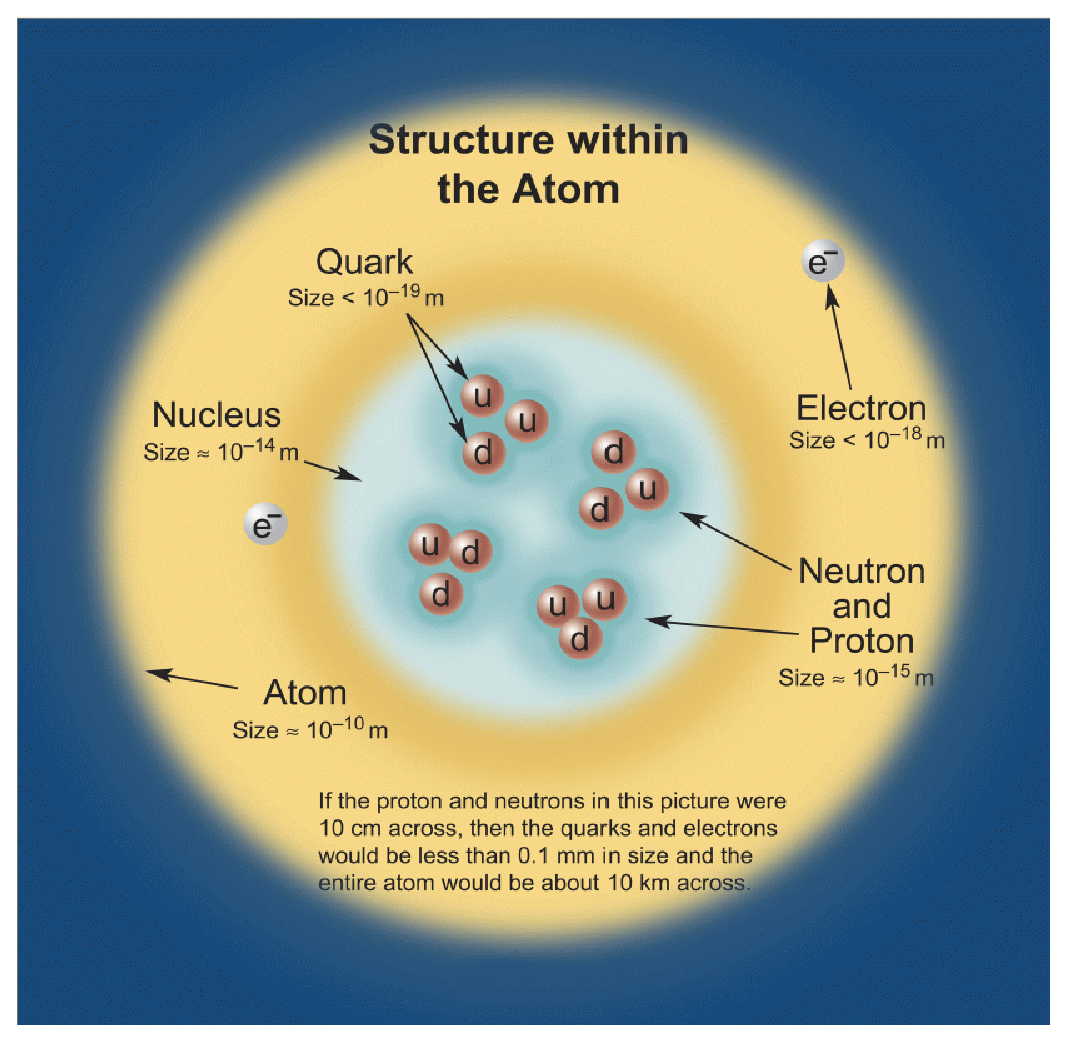
\includegraphics[width=3.4in]{AtomicStructure.ps}

\end{center}

\thispagestyle{empty}

\newpage


\ 
\setcounter{page}{1}

\vfill

Cover art: The atom consists of smaller electrons and a nucleus consisting of protons and neutrons.
The protons and neutrons, in turn, are formed from objects called quarks and gluons.
Courtesy, the American Institute of Physics.

\pagebreak

\tableofcontents{}

\newpage

\setcounter{page}{3}

\thispagestyle{plain}

\vfill

\ 

\pagebreak

\setcounter{activity}{0}

\section{Relating Position, Velocity, and Acceleration Graphs\footnote{
1990-93 Dept. of Physics and Astronomy, Dickinson College. Supported by FIPSE
(U.S. Dept. of Ed.) and NSF. Portions of this material may have been modified
locally and may not have been classroom tested at Dickinson College.
}}

Name \rule{2.0in}{0.1pt}\hfill{}Section \rule{1.0in}{0.1pt}\hfill{}Date \rule{1.0in}{0.1pt}

\textbf{Objective }

To understand the relationship between position vs. time, velocity vs. time, and acceleration vs. time
graphs.


\textbf{Introduction} 

The focus of this unit on kinematics is to be able to describe your position, velocity, and acceleration
as a function of time using words and graphs. You will use a motion detector
attached to a computer in the laboratory to learn to describe one-dimensional
motion.

The ultrasonic motion detector sends out a series of sound pulses that are of
too high a frequency to hear. These pulses reflect from objects in the vicinity
of the motion detector and some of the sound energy returns to the detector.
The computer is able to record the time it takes for reflected sound waves to
return to the detector and then, by knowing the speed of sound in air, figure
out how far away the reflecting object is. There are several things to watch
out for when using a motion detector. (1) Do not get closer than 0.15 meters
from the detector because it cannot record reflected pulses which come back
too soon. (2) The ultrasonic waves come out in a cone of about 15\( ^{\circ } \).
It will `see' the closest object. Be sure there is a clear path between the object
whose motion you want to track and the motion detector. (3) The motion detector
is very sensitive and will detect slight changes in motion. 
These changes will appear as bumps in your velocity vs. time graphs.

\vspace{5mm}

\textbf{Apparatus} 

\begin{table}[hbt]
\begin{tabular}{llll}
$\bullet$ & \textit{Science Workshop 750 Interface}  & $\bullet$ & Masking tape for marking distances  \\[3pt]
$\bullet$ & Ultrasonic motion detector               & $\bullet$ & Dynamics cart and track             \\[3pt]
$\bullet$ & \textit{DataStudio} software             & $\bullet$ & Lab stand to incline the track      \\[3pt]
$\bullet$ & Wooden board                             &                                                 \\[3pt]
\end{tabular}
\end{table}

\textbf{Position vs. Time Graphs of Your Motion }

The purpose of this activity is to learn how to relate graphs of position as a function
of time to the motions they represent. How does a position vs. time graph look
when you move slowly? Quickly? What happens when you move toward the motion
detector? Away? After completing the next few activities, you should be able
to look at a position vs. time graph and describe the motion of the object and sketch a graph
representing that motion.

Note that the motion detector measures the distance of an object from the detector,
and that the motion detector is located at the origin of each graph. It is common
to refer to the distance of an object from some origin as the position of the
object. Therefore, it is better to refer to these graphs as position vs. time
graphs than distance vs. time graphs.


\textbf{Activity \stepcounter{activity}\arabic{activity}: Making Position vs. Time Graphs }\actlabel{actone}

In this Activity you will measure your own movements with the motion sensor.
You can try to glide smoothly
along the floor, but don't be surprised to see small bumps in velocity graphs.
Also, some objects like bulky sweaters are good sound absorbers and may not be
``seen'' well by a motion detector. You may want to hold a book
or a board in front of you if you have loose clothing on.

You will use the \textit{DataStudio} software to do the following activities.
For Activity 1 launch the \textbf{Position
Graphs} application by going to \textbf{Start} $\rightarrow$ \textbf{Programs} $\rightarrow$ \textbf{Physics Applications} $\rightarrow$ \textbf{131 Workshop} $\rightarrow$ \textbf{Position Graphs}. To start a data run, click the \textbf{Start} button. To stop a data run,
click the \textbf{Stop} button. After a data run, the graph can be expanded
by clicking on the \textbf{Scale to fit} button in the upper left corner of
the Graph window. Multiple data sets can be displayed on the same graph. Data
can be removed from the graph by selecting \textbf{Delete Last Data Run} or
\textbf{Delete All Data Runs} from the \textbf{Experiment} menu. When you are
finished with the activities, choose \textbf{Quit} from the \textbf{File} menu
and do not save this activity.
See the Appendix for more details on using {\it DataStudio}.

Before you begin the activities, you should mark a position scale on the floor.
To do this, position one person at approximately 1 meter in front of the motion
detector and take data for 1 second. The computer will display a horizontal
line showing the position measured by the detector. The person standing in front
of the detector should then adjust his/her position and the procedure repeated
until the 1 meter position is established. Mark the 1 meter position on the
floor with a piece of masking tape and then mark the 2, 3 and 4 meter positions
using the 2 meter stick.

Make position-time graphs for the following motions and sketch the graph you
observe in each case:

\begin{enumerate}

\item Starting at 0.5 m, walk away from the origin (i.e., the detector) slowly
and steadily.

\vspace{0.3cm}
{\par\centering 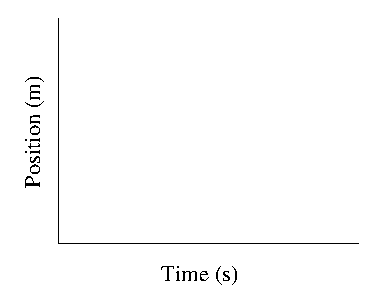
\includegraphics{iqsRelatingMotion/position_fig1.eps} \par}
\vspace{0.3cm}

\item Walk toward the detector (origin) quickly and steadily.

\vspace{0.3cm}
{\par\centering 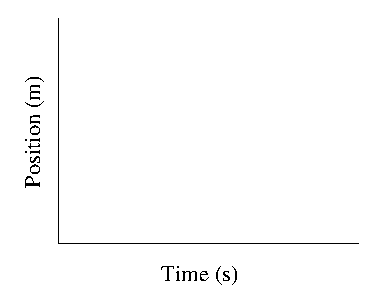
\includegraphics{iqsRelatingMotion/position_fig1.eps} \par}
\vspace{0.3cm}

\item Describe the difference between the graph made by walking toward and the
one made walking away from the motion detector.
\vspace{20mm}

\end{enumerate}

\newpage

\textbf{Activity \stepcounter{activity}\arabic{activity}: Predicting Velocity Graphs from Position Graphs}\actlabel{acttwo}

\begin{enumerate}

\item Carefully study the position graph shown below and predict the velocity
vs. time graph that would result from the motion. Using a dashed line, sketch
your prediction of the corresponding velocity vs. time graph on the velocity
axes.

\vspace{0.3cm}
{\par\centering 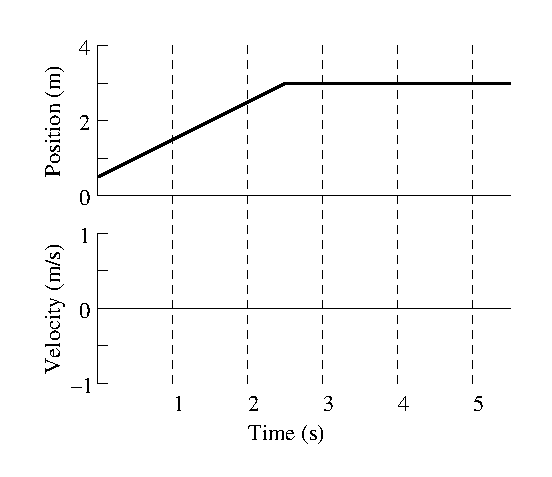
\includegraphics{iqsRelatingMotion/relating_fig1.eps} \par}
\vspace{0.3cm}

\item After each person in your group has sketched a prediction, test your prediction
by walking and matching the position vs. time graph shown. 
To explore how position vs. time and velocity vs. time graphs are related, 
go to \textbf{Start} $\rightarrow$ \textbf{Programs} $\rightarrow$ \textbf{Physics Applications} $
\rightarrow$ \textbf{131 Workshop} $\rightarrow$ \textbf{Position \& Velocity Graphs}.
When you have made a good duplicate
of the position graph, sketch your actual graph over the existing position vs.
time graph.
Use a solid line to draw the actual velocity graph on the same graph with
your prediction. (Do not erase your prediction).

\item How would the position graph be different if you moved faster? Slower? 
\vspace{20mm}

\item How would the velocity graph be different if you moved faster? Slower? 
\vspace{20mm}

\end{enumerate}

\newpage

\textbf{Activity \stepcounter{activity}\arabic{activity}: Finding Position from a Velocity Graph }\actlabel{actthree}

\begin{enumerate}

\item Carefully study the velocity graph that follows. Using a dashed line, sketch your prediction of the corresponding position graph on the top set of axes.
(Assume that you started at the 1-meter mark.)

\vspace{0.3cm}
{\par\centering 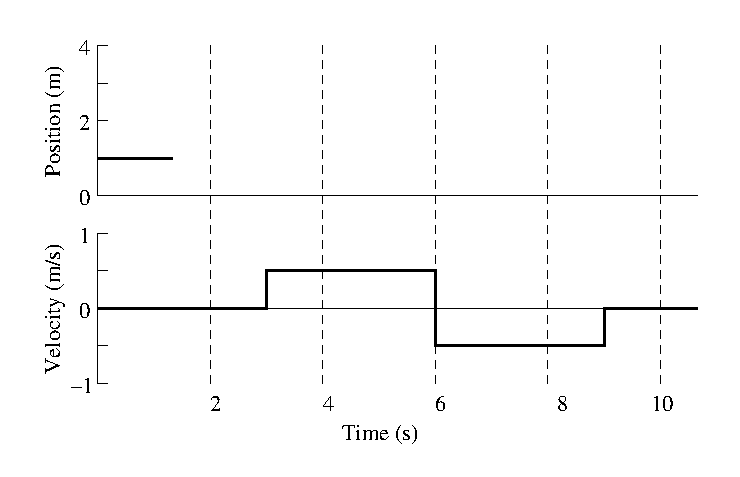
\includegraphics{iqsRelatingMotion/relating_fig2.eps} \par}
\vspace{0.3cm}

\item After each person has sketched a prediction, do your group's best to duplicate the bottom (velocity vs. time) graph by walking. 
When you have made a good duplicate of the velocity vs. time graph, draw your actual result over the existing velocity vs. time graph. 
Use a solid line on the top graph to draw the actual position vs. time graph on the same axes with your prediction. Do not erase your prediction.

\item How can you tell from a velocity vs. time graph that the moving object has
changed direction?
\vspace{10mm}

\item What is the velocity at the moment the direction changes? 
\vspace{10mm}

\item Is it possible to actually move your body (or an object) to make vertical
lines on a position vs. time graph? Why or why not? What would the velocity
be for a vertical section of a position vs. time graph? 
\vspace{10mm}

\item How can you tell from a position vs. time graph that your motion is steady
(motion at a constant velocity)? 
\vspace{10mm}

\item How can you tell from a velocity vs. time graph that your motion is steady
(constant velocity)? 
\vspace{10mm}

\end{enumerate}

\newpage

\textbf{Activity \stepcounter{activity}\arabic{activity}: Position, Velocity and Acceleration Graphs of Constant Velocity}\actlabel{actfour}

In order to get a feeling for acceleration, it is helpful to create and learn
to interpret velocity vs. time and acceleration vs. time graphs for some relatively
simple motions of a cart on a track. 
The cart's motion on a track is simpler than the more complex movements associated with walking.
You will be observing the cart with the
motion detector as it moves at a constant velocity and as it changes its velocity
at a constant rate. Use the \textbf{P, V \& A Graphs} application by going to
\textbf{Start} $\rightarrow$ \textbf{Programs} $\rightarrow$ \textbf{Physics Applications} 
$\rightarrow$ \textbf{131 Workshop} $\rightarrow$ \textbf{P, V \& A Graphs} for these activities.

\begin{enumerate}

\item Based on your observations of the motions of your body in the last Activity,
how should the position and velocity graphs look if you move the cart at a constant
velocity away from the motion detector starting at the 0.5 meter mark? Sketch
your predictions with dashed lines on the axes that follow.

%\vspace{0.3cm}
{\par\centering 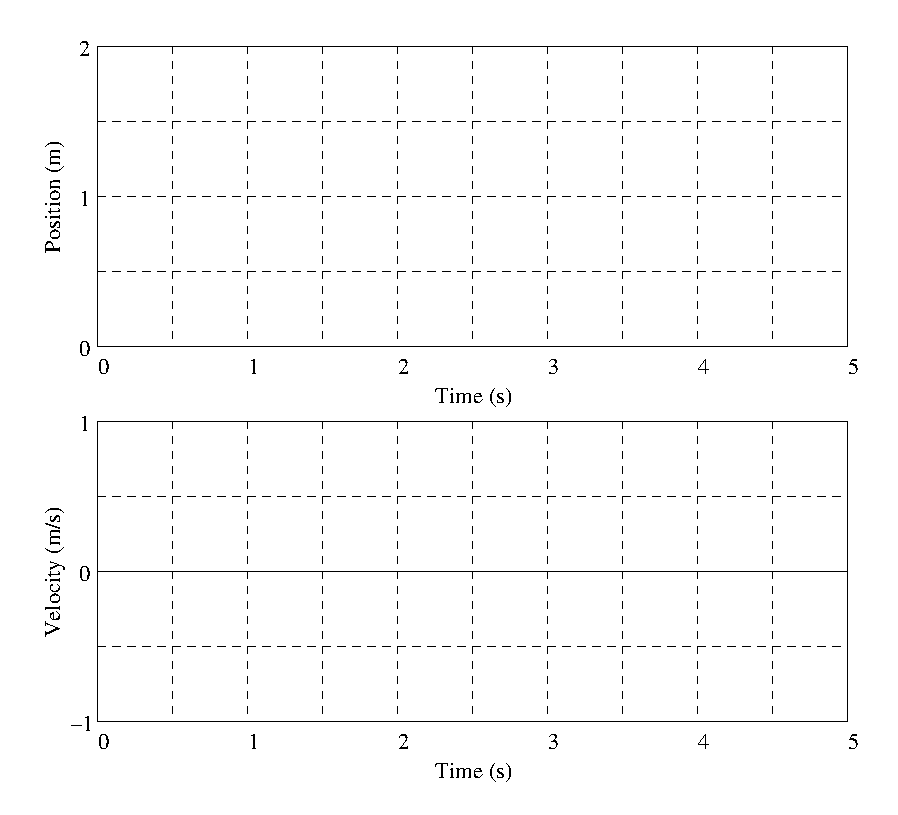
\includegraphics[width=4.75in]{iqsRelatingMotion/changing_fig1.eps} \par}
\vspace{0.1cm}

\item Acceleration is defined as the time rate of change of velocity. Sketch your
prediction of the cart acceleration on the axes that follow using a dashed line.

%\vspace{0.3cm}
{\par\centering 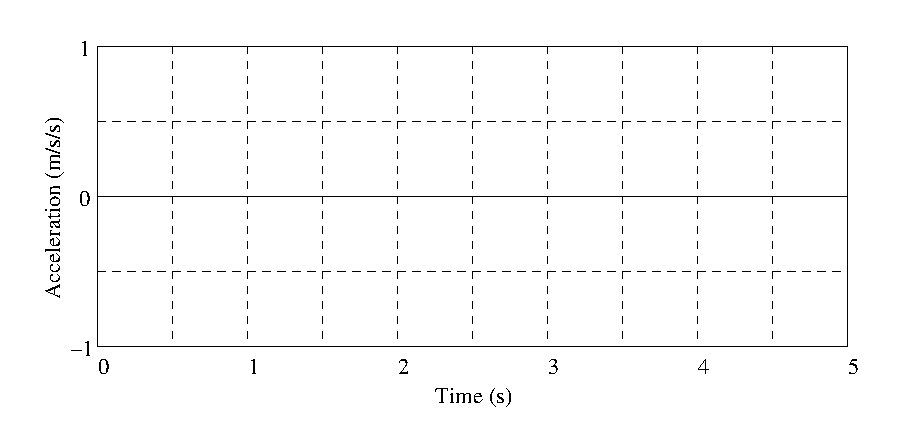
\includegraphics[width=4.75in]{iqsRelatingMotion/changing_fig2.eps} \par}
\vspace{0.1cm}

\item Test your prediction. Be sure that the cart is never closer than 0.15 meter
from the motion detector. Try several times until you get a fairly constant
velocity. Sketch your results with solid lines on the axes shown above. The
acceleration vs. time graphs will exhibit small fluctuations due to irregularities
in the motion of the cart. You should ignore these fluctuations and draw smooth
patterns.

\item Did your graphs agree with your predictions? What characterizes constant
velocity motion on a position vs. time graph? 
\vspace{10mm}

\item What characterizes constant velocity motion on a velocity vs. time graph?
\vspace{10mm}

\item What characterizes constant velocity motion on an acceleration vs. time graph?
\vspace{10mm}

\end{enumerate}

\textbf{Speeding Up at a Moderate Rate} 

In the next activity you will look at velocity and acceleration graphs of the
motion of a cart when its velocity is changing. You will be able to see how
these two representations of the motion are related to each other when the cart
is speeding up.
In order to get your cart speeding up smoothly use the lab stand to raise the
track several centimeters at the end where the motion detector is mounted.

\textbf{Activity \stepcounter{activity}\arabic{activity}: Graphs Depicting Speeding Up}\actlabel{actsix}

\begin{enumerate}

\item Predict the shape of the position, velocity, and acceleration vs. time graphs
for the cart moving away from the sensor and speeding up. Sketch your predictions
on the following axes using dashed lines.

\vspace{0.3cm}
{\par\centering 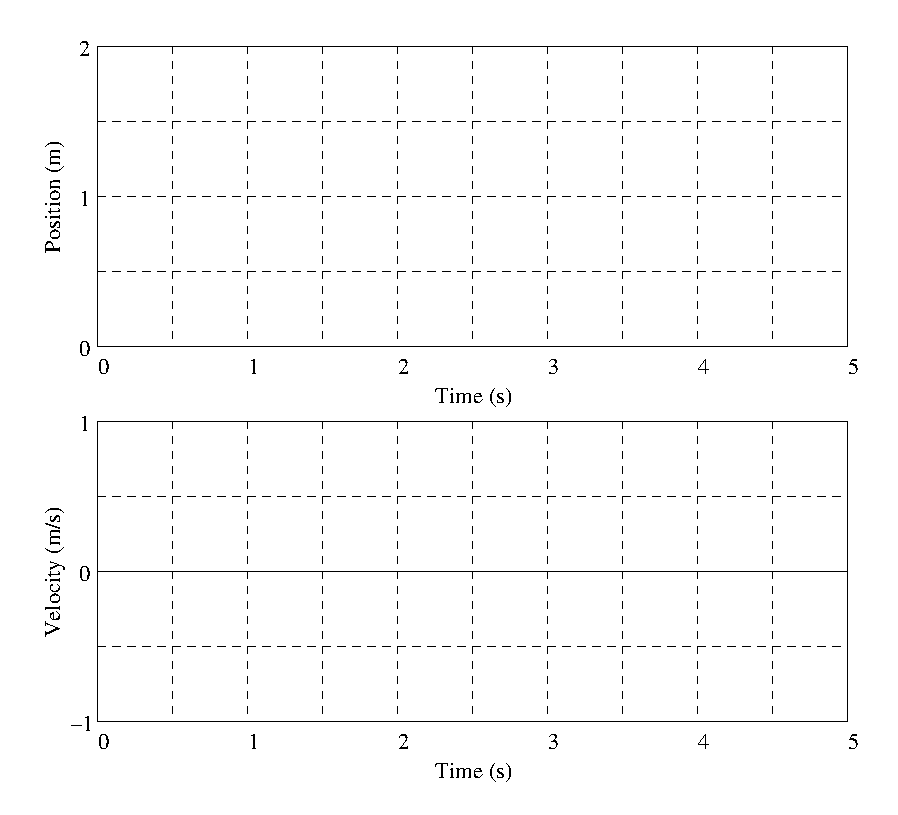
\includegraphics[width=4.75in]{iqsRelatingMotion/changing_fig1.eps} \par}
\vspace{0.3cm}

\vspace{0.3cm}
{\par\centering 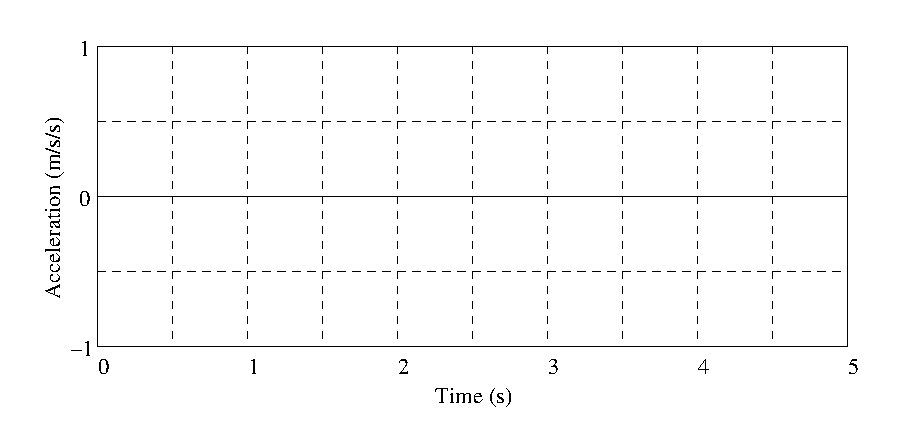
\includegraphics[width=4.75in]{iqsRelatingMotion/changing_fig2.eps} \par}
\vspace{0.3cm}

\item Create graphs of the motion of your cart as it moves away from the detector
and speeds up. Sketch the graphs neatly on the above axes using solid lines.

\item How does your position graph differ from the position graphs for steady
(constant velocity) motion? 
\vspace{13mm}

\item What feature of your velocity graph signifies that the motion was away from
the detector? 
\vspace{13mm}

\item What feature of your velocity graph signifies that the cart was speeding
up? How would a graph of motion with a constant velocity differ? 
\vspace{13mm}

\item During the time that the cart is speeding up, is the acceleration positive
or negative? How does speeding up while moving away from the detector result
in this sign of acceleration? Hint: Remember that acceleration is the rate of
change of velocity. Look at how the velocity is changing.\customlabel{posneg}{6}
\vspace{13mm}

\item How does the velocity vary in time as the cart speeds up? Does it increase
at a steady rate or in some other way? 
\vspace{13mm}

\item How does the acceleration vary in time as the cart speeds up? Is this what
you expect based on the velocity graph? Explain.
\vspace{13mm}

\end{enumerate}

\newpage

\textbf{Homework} 

\begin{enumerate}

\item To find the average acceleration of the cart during some time interval (the
average time rate of change of its velocity), you must measure its velocity
at two different times, calculate the difference between the final value and
the initial value and divide by the time interval.
Calculate the average acceleration during some time interval from your velocity graph in Activity \ref{actfour}.  
Does the result agree with your acceleration graph in Activity \ref{actfour}?
\vspace{20mm}

\item The diagram below shows the positions of the cart at equal time intervals.
(This is like taking snapshots of the cart at equal time intervals.) At each
indicated time, sketch a vector above the cart which might represent the velocity
of the cart at that time while it is moving at a constant velocity away from
the motion detector.

\vspace{0.3cm}
{\par\centering 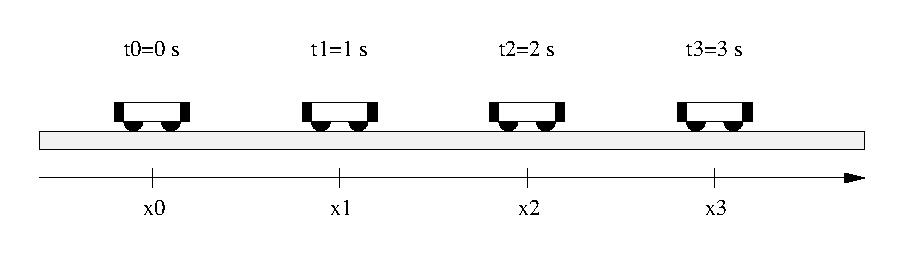
\includegraphics{iqsRelatingMotion/changing_fig3.eps} \par}
\vspace{0.3cm}

\item Explain how you would find the vector representing the change in velocity
between the times 1.0~s and 2.0~s in the diagram above. From this vector, what
value would you calculate for the acceleration? Explain. Is this value in agreement
with the acceleration graph you obtained in Activity \ref{actfour}?
\vspace{20mm}


\item  The diagram below shows the positions of the cart at equal time intervals.
At each indicated time, sketch a vector above the cart which might represent
the velocity of the cart at that time while it is moving away from the motion
detector and speeding up.

\vspace{0.3cm}
{\par\centering 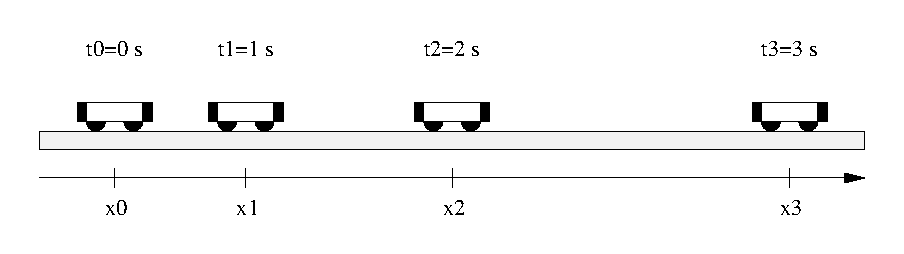
\includegraphics{iqsRelatingMotion/changing_fig4.eps} \par}
\vspace{0.3cm}

\newpage

Show below how you would find the approximate length and direction of the
vector representing the change in velocity between the times 1.0~s and 2.0~s
using the diagram above. No quantitative calculations are needed. Based on the
direction of this vector and the direction of the positive x-axis, what is the
sign of the acceleration? Does this agree with your answer to Activity \ref{actsix}.\ref{posneg}?
\vspace{20mm}

\item Draw the velocity graphs for an object whose motion produced the position-time
graphs shown below on the left. Position is in meters and velocity in meters
per second. Note: Unlike most real objects, you can assume these objects can
change velocity so quickly that it looks instantaneous with this time scale.

%\vspace{0.3cm}
%{\par\centering 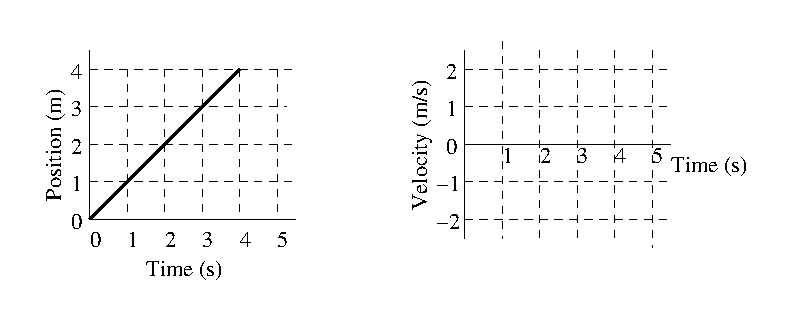
\includegraphics{iqsRelatingMotion/relating_fig3.eps} \par}
%\vspace{0.3cm}

\vspace{0.3cm}
{\par\centering 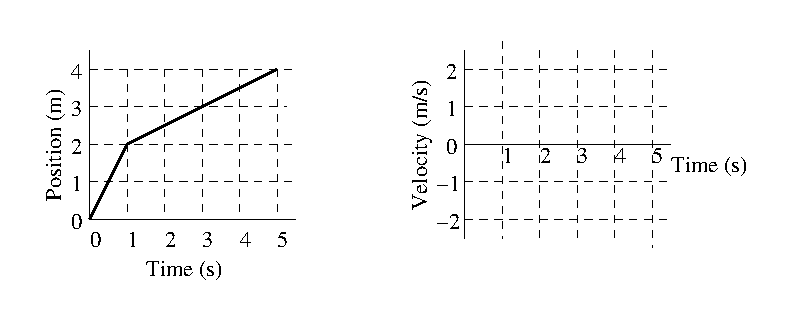
\includegraphics{iqsRelatingMotion/relating_fig4.eps} \par}
\vspace{0.3cm}

\vspace{0.3cm}
{\par\centering 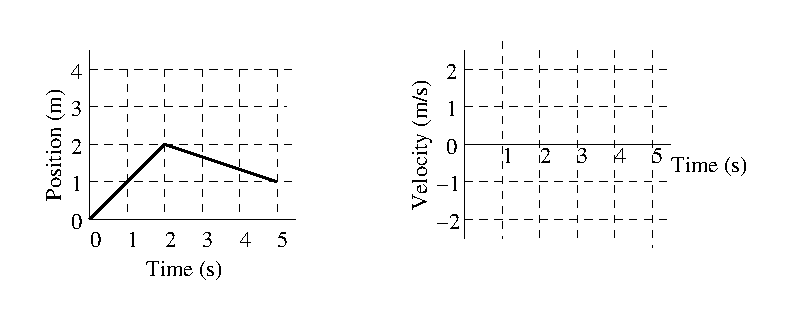
\includegraphics{iqsRelatingMotion/relating_fig5.eps} \par}
\vspace{0.3cm}

\newpage

\item Draw careful graphs below of position and velocity for a cart that (a) moves
away from the origin at a slow and steady (constant) velocity for the first
5 seconds; (b) moves away at a medium-fast, steady (constant) velocity for the
next 5 seconds; (c) stands still for the next 5 seconds; (d) moves toward the
origin at a slow and steady (constant) velocity for the next 5 seconds; (e)
stands still for the last 5 seconds.

\vspace{0.3cm}
{\par\centering 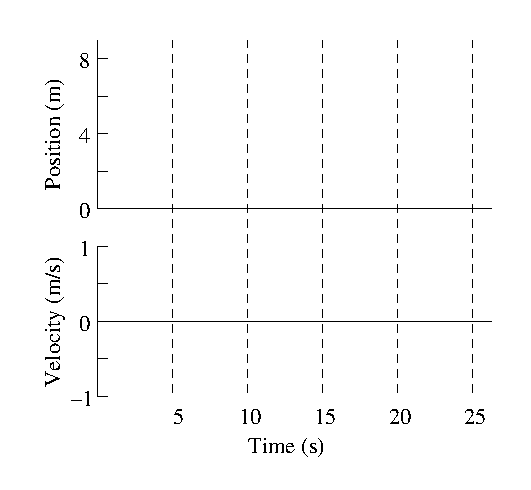
\includegraphics{iqsRelatingMotion/relating_fig6.eps} \par}
\vspace{0.3cm}


\item An object moving along a line (the + position axis) has the acceleration-time
graph shown below. Describe how might the object move to create this graph if
it is moving away from the origin?

\vspace{0.3cm}
{\par\raggedright 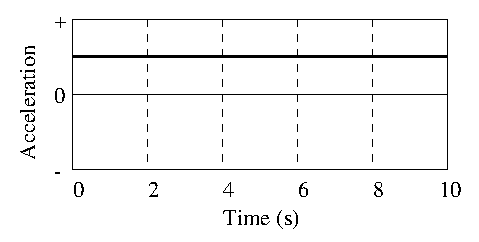
\includegraphics{iqsRelatingMotion/changing_fig6.eps} \par}
\vspace{1.3cm}

\item Sketch on the axes below a velocity-time graph that goes with the above acceleration-time
graph.

\vspace{0.3cm}
{\par\centering 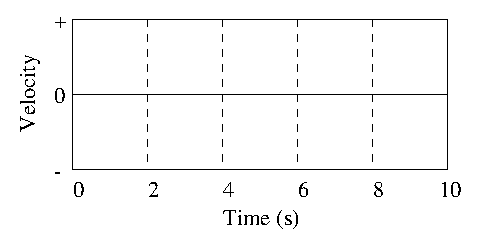
\includegraphics{iqsRelatingMotion/changing_fig7.eps} \par}
\vspace{1.3cm}

\item For each of the velocity-time graphs below, sketch the shape of the acceleration-time
graph that goes with it.

\vspace{0.3cm}
{\par\centering 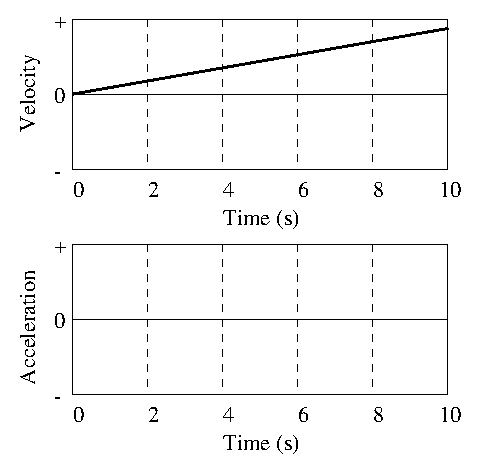
\includegraphics{iqsRelatingMotion/changing_fig8.eps} \par}
\vspace{0.3cm}

\vspace{0.3cm}
{\par\centering 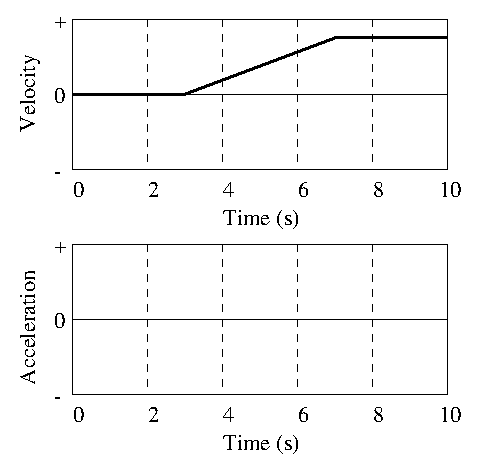
\includegraphics{iqsRelatingMotion/changing_fig9.eps} \par}
\vspace{0.3cm}

%\item The following is a velocity-time graph for a car.

%\vspace{0.3cm}
%{\par\centering 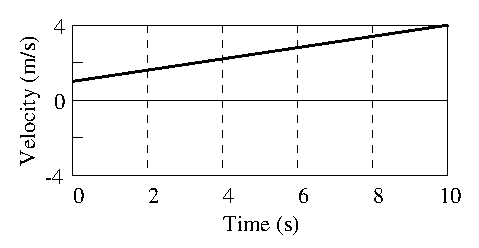
\includegraphics{iqsRelatingMotion/changing_fig10.eps} \par}
%\vspace{0.3cm}

%What is the average acceleration of the car? Show your work below.
%\vspace{30mm}

\item Which position-time graph below could be that for a cart that is steadily
accelerating away from the origin?

\vspace{0.3cm}
{\par\centering 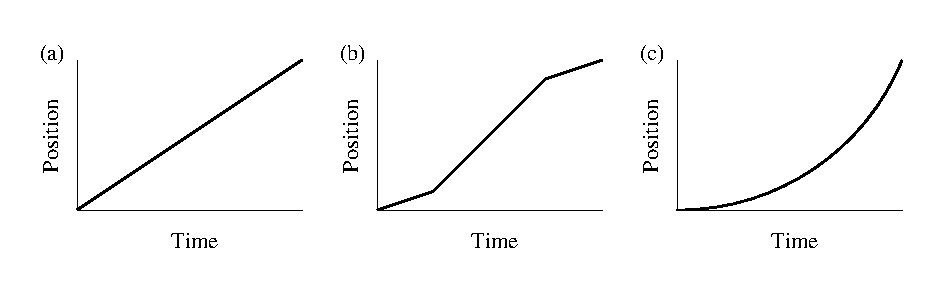
\includegraphics{iqsRelatingMotion/changing_fig11.eps} \par}
\vspace{0.3cm}


\item A car can move along a line (the + position axis). Sketch velocity-time and
acceleration-time graphs which correspond to each of the following descriptions
of the car's motion.
The car starts from rest and moves away from the origin increasing its speed
at a steady rate.

\vspace{0.3cm}
{\par\centering 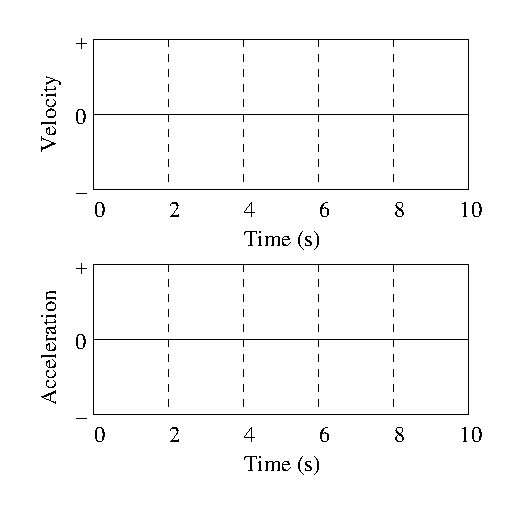
\includegraphics{iqsRelatingMotion/changing_fig12.eps} \par}
\vspace{0.3cm}

\item The same car is moving away from the origin at a constant velocity.

\vspace{0.3cm}
{\par\centering 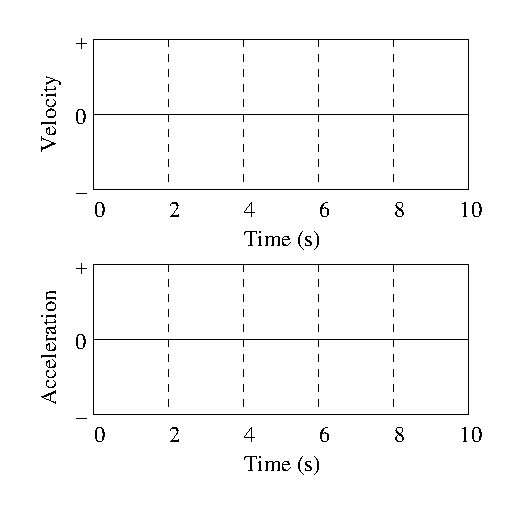
\includegraphics{iqsRelatingMotion/changing_fig12.eps} \par}
\vspace{0.3cm}

%\item The car starts from rest and moves away from the origin increasing its speed
%at a steady rate twice as large as in (6) above.

%\vspace{0.3cm}
%{\par\centering 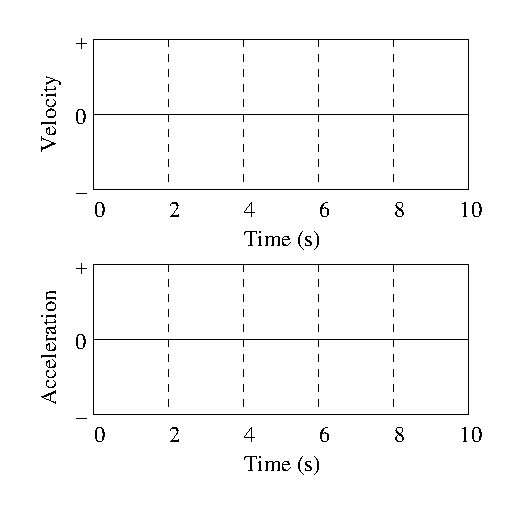
\includegraphics{iqsRelatingMotion/changing_fig12.eps} \par}
%\vspace{0.3cm}

%\item The car is moving away from the origin at a constant velocity twice as large
%as in (7) above.

%\vspace{0.3cm}
%{\par\centering 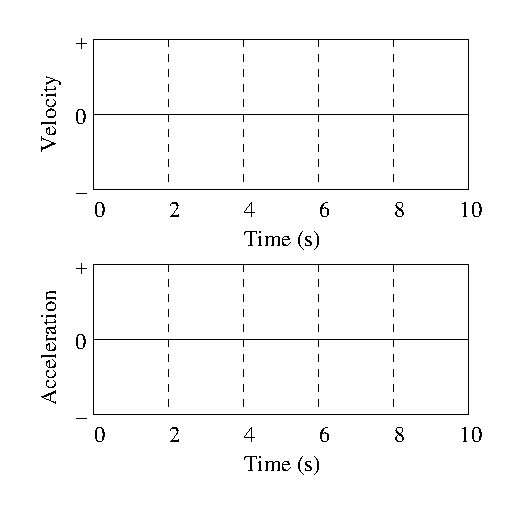
\includegraphics{iqsRelatingMotion/changing_fig12.eps} \par}
%\vspace{0.3cm}

\end{enumerate}


%\include{changing}

\setcounter{activity}{0}

\section{Slowing Down, Speeding Up, and Turning\footnote{
1990-93 Dept. of Physics and Astronomy, Dickinson College. Supported by FIPSE
(U.S. Dept. of Ed.) and NSF. Portions of this material may have been modified
locally and may not have been classroom tested at Dickinson College.
}}

Name \rule{2.0in}{0.1pt}\hfill{}Section \rule{1.0in}{0.1pt}\hfill{}Date \rule{1.0in}{0.1pt}

\textbf{Objectives }

\begin{itemize}
\item To learn how to relate graphs of acceleration vs. time to the motions they represent. 
\item To understand the relationship between velocity vs. time and acceleration vs.
time graphs.
\end{itemize}
\textbf{About Slowing Down, Speeding Up and Turning }

In the previous session, you explored the characteristics of position vs. time,
velocity vs. time and acceleration vs. time graphs of the motion of a dynamics
cart. In the cases examined, the cart was always moving away from a motion detector,
either at a constant velocity or with a constant acceleration. Under these conditions,
the velocity and acceleration are both positive. You also learned how to find
the magnitude of the acceleration from velocity vs. time and acceleration vs.
time graphs, and how to represent the velocity and acceleration using vectors. 

In the motions you studied in the last session, the velocity and acceleration
vectors representing the motion of the cart both pointed in the same direction.
In order to get a better feeling for acceleration, it will be helpful to examine
velocity vs. time and acceleration vs. time graphs for some slightly more complicated
motions of a cart on an inclined track. Again you will use the motion detector
to observe the cart as it changes its velocity at a constant rate. Only this
time the motion may be toward the detector, and the cart may be speeding up
or slowing down.

\textbf{Apparatus }

\begin{itemize}
\item \textit{Science Workshop 750 Interface}
\item Ultrasonic motion detector 
\item \textit{DataStudio} software (P, V \& A Graphs application)
\item Dynamics cart and track 
\item Lab stand to incline the track
\end{itemize}
\textbf{Slowing Down and Speeding Up }

In this activity you will look at a cart moving along an inclined track and
slowing down. A car being brought to rest by the steady action of brakes is
a good example of this type of motion. Later you will examine the motion of
the cart toward the motion detector and speeding up. In both cases, we are interested
in the shapes of the velocity vs. time and acceleration vs. time graphs, as
well as the vectors representing velocity and acceleration. 

Let's start with the creation of velocity and acceleration graphs of when it
is moving away from the motion detector and slowing down. To do this activity,
the track should be inclined with a lab stand at one end and the motion detector set up at the lower end of the track. Adjust the lab stand so that the track is raised a few centimeters at the opposite end from where the motion detector is located. Now when you give the cart a push away from the motion detector, it will slow down after it is released. In this activity you will examine the velocity and acceleration of this motion.

\textbf{Activity \stepcounter{activity}\arabic{activity}: Graphs Depicting Slowing Down} \actlabel{slowingone}

(a) If you give the cart a push away from the motion detector and release it,
will the acceleration be positive, negative or zero (after it is released)?
Sketch your predictions for the velocity vs. time and acceleration vs. time
graphs on the axes below using dashed lines.

\vspace{0.3cm}
{\par\centering 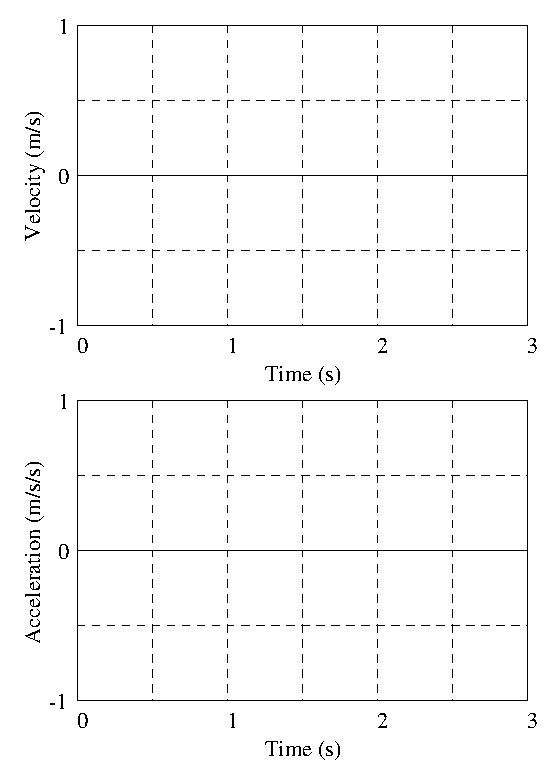
\includegraphics{slowing/slowing_fig1.eps} \par}
\vspace{0.3cm}

(b) To test your predictions, open the \textbf{P, V \& A Graphs} application. Locate the cart 0.15 m from the motion detector and gently push the cart away from the motion detector once it starts clicking. Catch the cart \underline{before} it turns around or hits the end of the track.

Draw the results on the axes above using solid lines for the part of the motion
after the cart is released. You may have to try a few times to get a good run.  The acceleration vs. time graphs will exhibit small fluctuations due to irregularities in the motion of the cart. You should ignore these fluctuations and draw smooth patterns.

(c) Did the shapes of your velocity and acceleration graphs agree with your
predictions? How is the sign of the acceleration represented on a velocity vs.
time graph? 
\vspace{20mm}

(d) How is the sign of the acceleration represented on an acceleration vs. time
graph? 
\vspace{20mm}

\newpage

(e) Is the sign of the acceleration what you predicted? How does slowing down
while moving away from the detector result in this sign of acceleration? Hint:
Remember that acceleration is the rate of change of velocity. Look at how the
velocity is changing.
\vspace{20mm}

\textbf{Constructing Acceleration Vectors for Slowing Down }

Let's consider a diagrammatic representation of a cart which is slowing down
and use vector techniques to figure out the direction of the acceleration.

\textbf{Activity \stepcounter{activity}\arabic{activity}: Vector Diagrams for Slowing Down}\actlabel{slowingtwo}

(a) The diagram that follows shows the positions of the cart at equal time intervals.
(This is like taking snapshots of the cart at equal time intervals.) At each
indicated time, sketch a vector above the cart which might represent the velocity
of the cart at that time while it is moving away from the motion detector and
slowing down.

\vspace{0.3cm}
{\par\centering 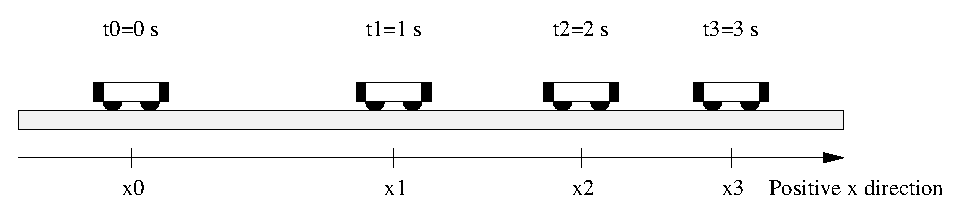
\includegraphics{slowing/slowing_fig2.eps} \par}
\vspace{0.3cm}


(b) Show below how you would find the vector representing the change in velocity
between the times 1s and 2 s in the diagram above. Based on the direction of
this vector and the direction of the positive x-axis, what is the sign of the
acceleration? Does this agree with your answer to Question (e) in Activity \ref{slowingone}?
\vspace{20mm}

(c) Based on your observations in this activity and in the last session, state
the general rules to predict the sign and direction of the acceleration if you
know the sign of the velocity (i.e., the direction of motion) and whether the
object is speeding up or slowing down.
\vspace{25mm}

\textbf{Speeding Up Toward the Motion Detector} 

Let's investigate another common situation. Suppose the cart is allowed to speed up when traveling toward the motion detector. What will be the direction of the acceleration? Positive or negative? 

\textbf{Activity \stepcounter{activity}\arabic{activity}: Graphs Depicting Speeding Up} \actlabel{slowingthree}

(a) Use the general rules that you stated in Activity \ref{slowingtwo} to predict the shapes
of the velocity and acceleration graphs. Sketch your predictions using dashed
lines on the axes that follow.

\vspace{0.3cm}
{\par\centering 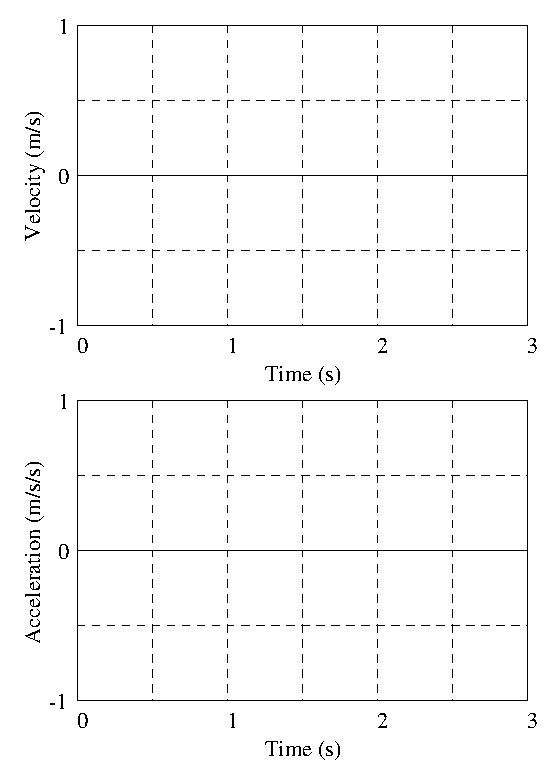
\includegraphics{slowing/slowing_fig1.eps} \par}
\vspace{0.3cm}

(b) Test your predictions by releasing the cart from rest at the raised end of the track after the motion detector starts clicking. Catch the cart before it gets too close to the detector.

Draw the results using solid lines on the axes above. You may have to try a
few times to get a good run.

(c) How does your velocity graph show that the cart was moving toward the detector? 
\vspace{20mm}

(d) During the time that the cart was speeding up, is the acceleration positive
or negative? Does this agree with your prediction? Explain how speeding up while
moving toward the detector results in this sign of acceleration. Hint: Think
about how the velocity is changing.
\vspace{20mm}

\textbf{Constructing Acceleration Vectors for Speeding Up} 

Let's consider a diagrammatic representation of a cart which is speeding up
and use vector techniques to figure out the direction of the acceleration.

\vspace{10mm}

\textbf{Activity \stepcounter{activity}\arabic{activity}: Vector Diagrams for Speeding Up} \actlabel{slowingfour}

(a) The diagram that follows shows the positions of the cart at equal time intervals.
(This is like taking snapshots of the cart at equal time intervals.) At each
indicated time, sketch a vector above the cart which might represent the velocity
of the cart at that time while it is moving toward the motion detector and speeding
up.

\vspace{0.3cm}
{\par\centering 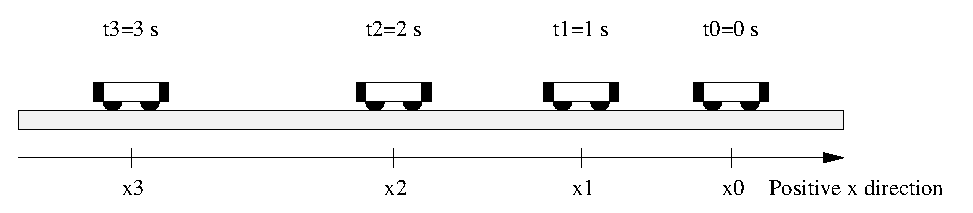
\includegraphics{slowing/slowing_fig3.eps} \par}
\vspace{0.3cm}

(b) Show below how you would find the vector representing the change in velocity
between the times 1s and 2 s in the diagram above. Based on the direction of
this vector and the direction of the positive x-axis, what is the sign of the
acceleration? Does this agree with your answer to Question (d) in Activity \ref{slowingthree}?
\vspace{20mm}

\textbf{Moving Toward the Detector and Slowing Down }

There is one more possible combination of velocity and acceleration for the
cart, that of moving toward the detector while slowing down. 

\textbf{Activity \stepcounter{activity}\arabic{activity}: Slowing Down Toward the Detector}\actlabel{slowingfive}

(a) Use your general rules to predict the direction and sign of the acceleration
when the cart is slowing down as it moves toward the detector. Explain why the
acceleration should have this direction and this sign in terms of the velocity
and how the velocity is changing. 
\vspace{20mm}

(b) The diagram below shows the positions of the cart at equal time intervals
for slowing down while moving toward the detector. At each indicated time, sketch
a vector above the cart which might represent the velocity of the cart at that
time while it is moving toward the motion detector and slowing down.

\vspace{0.3cm}
{\par\centering 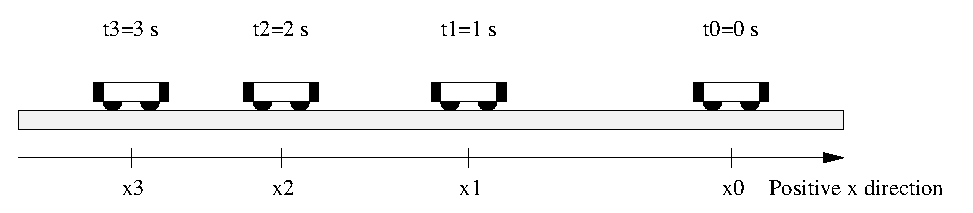
\includegraphics{slowing/slowing_fig4.eps} \par}
\vspace{0.3cm}

\newpage %%%%%%%%%%%%%%%%%%%%%%%%%%%%%%%%%%%%%%%%%%%%%%%%%%%%%%%%%%

(c) Show below how you would find the vector representing the change in velocity
between the times 1s and 2 s in the diagram above. Based on the direction of
this vector and the direction of the positive x-axis, what is the sign of the
acceleration? Does this agree with the prediction you made in part (a)?
\vspace{15mm}

\textbf{Acceleration and Turning Around }

In some recent Activities, you looked at
velocity vs. time and acceleration vs. time graphs for a cart moving in one
direction with a changing velocity. In this investigation you will look at what
happens when the cart slows down, turns around and then speeds up. (This is a
combination of Activities 1 and 3.)

To practice this motion you should position the cart 0.15 m from the detector
and give the cart a gentle push away from the motion detector. It should move
up the track, slow down, reverse direction and then move back down toward the
detector. Try it without activating the motion detector! Be sure that the cart
does not hit the end of the track before it turns around. 

\textbf{Activity \stepcounter{activity}\arabic{activity}: Reversing Direction }\actlabel{slowingsix}

(a) For each part of the motion-away from the detector, at the turning point,
and toward the detector, predict in the table that follows whether the velocity
will be positive, zero or negative. Also indicate whether the acceleration is
positive, zero or negative.

\vspace{0.3cm}
{\centering \begin{tabular}{|c|c|c|c|}
\hline 
&
Moving Away&
Turning Around&
Moving Toward\\
\hline 
Velocity&
&
&
\\
\hline 
Acceleration&
&
&
\\
\hline 
\end{tabular}\par}
\vspace{0.3cm}

(b) Sketch the predicted shapes of the velocity vs. time and acceleration vs.
time graphs of this entire motion on the axes that follow using dashed lines.

\vspace{0.3cm}
{\par\centering 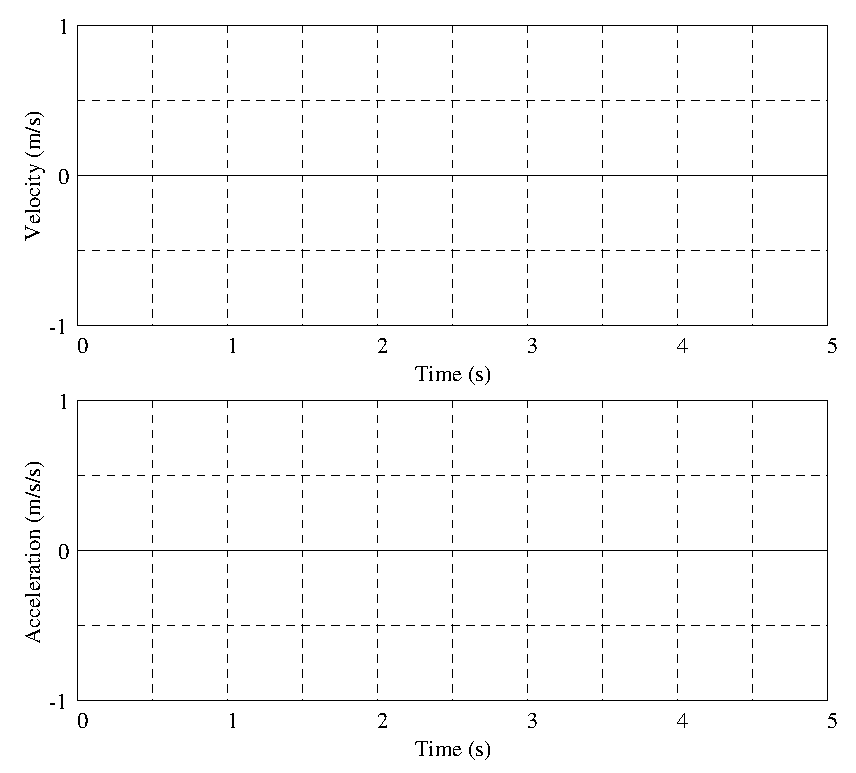
\includegraphics{slowing/slowing_fig5.eps} \par}
\vspace{13mm}

(c) Test your predictions by making graphs of the motion. Use the procedures
you used in the slowing down and speeding up activities. You may have to try
a few times to get a good run. When you get a good run, sketch both graphs on the axes above using solid lines.
Print your results from {\it DataStudio} and attach them to this unit.

(d) Did the cart have a zero velocity at any point in the motion? (Hint: Look
at the velocity graph. What was the velocity of the cart at the end of the ramp?)
Does this agree with your prediction? How much time did it spend at zero velocity
before it started back toward the detector?
\vspace{20mm}

(e) According to your acceleration graph, what is the acceleration at the instant
the cart comes to rest? Is it positive, negative or zero? Does this agree with
your prediction? 
\vspace{20mm}

\newpage

(f) Explain the observed sign of the acceleration at the end of the ramp. (Hint: Remember that acceleration is the rate of change of velocity.) 
\vspace{20mm}

(g) Print a copy of the position, velocity, and acceleration graphs for each person in your group and add the graphs to this unit.

(h) Notice that the slope of the velocity graph is not quite the same for positive velocities as it is for negative velocities. (This difference can also be seen on the acceleration graph.) What accounts for this difference?
\vspace{20mm}

\begin{comment}
\textbf{Tossing a Ball }

Suppose you throw a ball up into the air. It moves upward, reaches its highest
point and then moves back down toward your hand. We will now consider what can be said about the directions of its velocity and acceleration vectors at various points.

\textbf{Activity \stepcounter{activity}\arabic{activity}: The Rise and Fall of a Ball} \actlabel{slowingseven}

(a) Consider the ball toss carefully. Assume that upward is the positive direction.
Indicate in the table that follows whether the velocity is positive, zero or
negative during each of the three parts of the motion. Also indicate if the
acceleration is positive, zero or negative. Hint: Remember, to find the acceleration
you must look at the change in velocity.

\vspace{0.3cm}
{\centering \begin{tabular}{|c|c|c|c|}
\hline 
&
Moving Up&
At Highest Point&
Moving Down\\
&
(After Release)&
&
\\
\hline 
Velocity&
&
&
\\
\hline 
Acceleration&
&
&
\\
\hline 
\end{tabular}\par}
\vspace{0.3cm}

(b) In what ways is the motion of the ball similar to the motion of the cart
which you just observed?
\vspace{20mm}
\end{comment}

\textbf{Homework} 

1. An object moving along a line (the + position axis) has the acceleration-time graph below. How might the object move to create this graph if it is moving
toward the origin?

\vspace{0.3cm}
{\par\centering 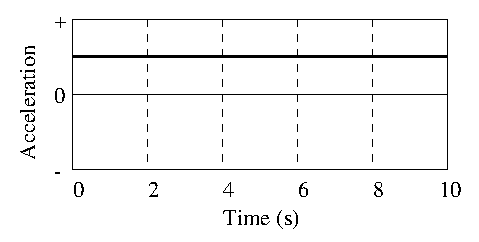
\includegraphics{slowing/slowing_fig6.eps} \par}
\vspace{0.3cm}

2. Sketch on the axes below the velocity-time graph that goes with the above
acceleration- time graph.

\vspace{0.3cm}
{\par\centering 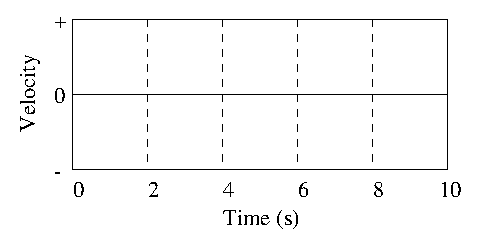
\includegraphics{slowing/slowing_fig7.eps} \par}
\vspace{0.3cm}

3. How would an object move to create each of the three labeled parts of the
acceleration-time graph shown below? (Consider the labeled straight line segments only, not the connectors between them.)

\vspace{0.3cm}
{\par\centering 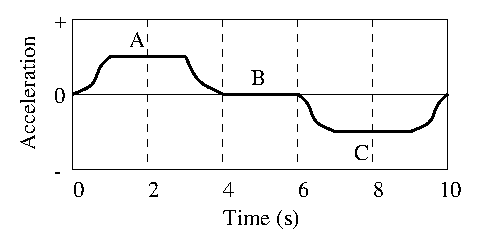
\includegraphics{slowing/slowing_fig8.eps} \par}
\vspace{0.3cm}

A: 
\vspace{10mm}

B: 
\vspace{10mm}

C:
\vspace{30mm}

4. Sketch below a velocity-time graph which might go with the acceleration-time
graph in question (3). (Again, consider the straight line segments only.)

\vspace{0.3cm}
{\par\centering 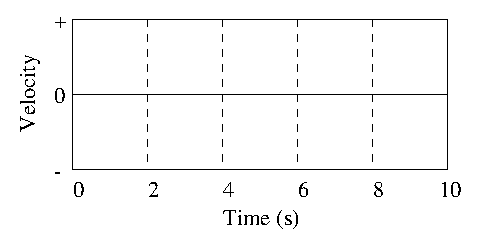
\includegraphics{slowing/slowing_fig9.eps} \par}
\vspace{0.3cm}

5. Sketch the shape of the acceleration-time graph that goes with the velocity-time
graph shown below.

\vspace{0.3cm}
{\par\centering 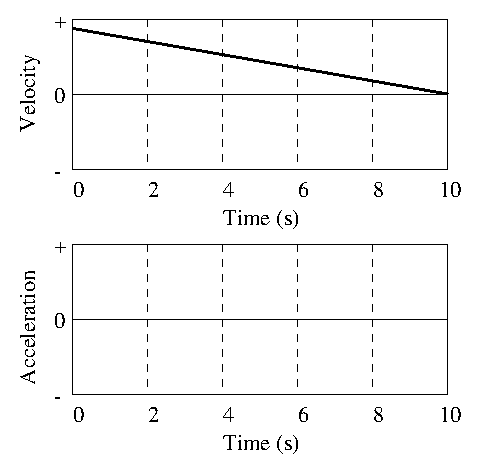
\includegraphics{slowing/slowing_fig10.eps} \par}
\vspace{0.3cm}

\newpage 

6. A car moves along a line {[}the + position axis{]}. Fill in the table below
with the sign (+ or -) of the velocity and acceleration of the car for each
of the motions described.

\vspace{0.3cm}
{\centering \begin{tabular}{|c|c|c|c|c|}
\hline 
&
Position&
Velocity&
Acceleration&
Acceleration\\
&
&
&
Speeding Up&
Slowing Down\\
\hline 
Car Moves Away&
+&
&
&
\\
from the Origin&
&
&
&
\\
\hline 
Car Moves Toward&
+&
&
&
\\
the Origin&
&
&
&
\\
\hline 
\end{tabular}\par}
\vspace{0.3cm}

7. Describe how you would move to produce the velocity-time graph shown below.

\vspace{0.3cm}
{\par\raggedright 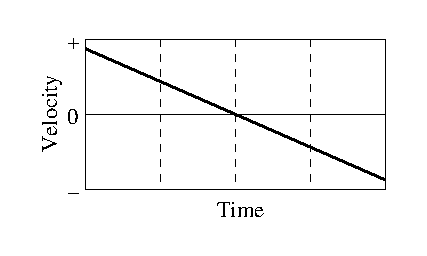
\includegraphics{slowing/slowing_fig12.eps} \par}
\vspace{0.3cm}

8. Sketch a position-time graph corresponding to the velocity-time graph above.

\vspace{0.3cm}
{\par\centering 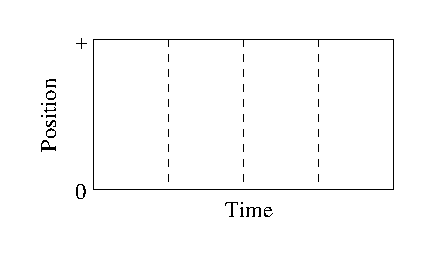
\includegraphics{slowing/slowing_fig13.eps} \par}
\vspace{0.3cm}

9. Sketch an acceleration-time graph corresponding to the velocity-time graph
above.

\vspace{0.3cm}
{\par\centering 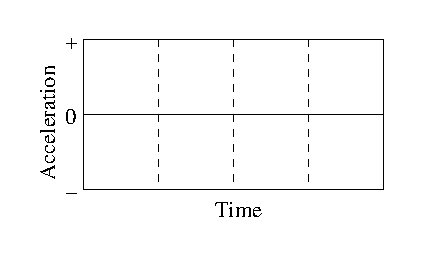
\includegraphics{slowing/slowing_fig14.eps} \par}
\vspace{0.3cm}

\newpage

10. For each of the position-time graphs shown, sketch below it the corresponding
velocity- time and acceleration-time graphs.

\vspace{0.3cm}
{\par\centering 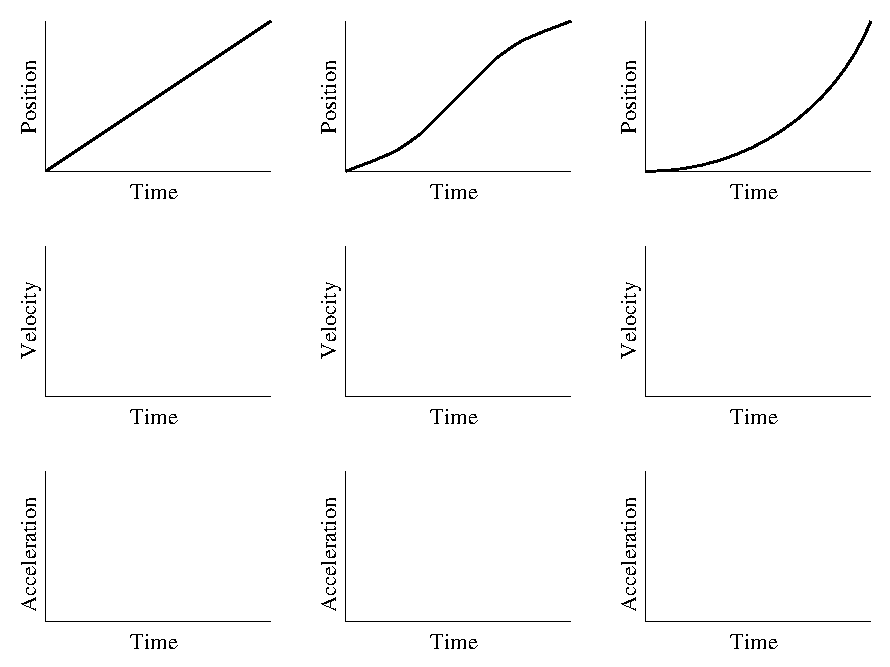
\includegraphics{slowing/slowing_fig11.eps} \par}
\vspace{0.3cm}

A car can move in either direction along a line (the + position axis). Sketch
velocity-time and acceleration-time graphs that correspond to each of the following
descriptions of the car's motion.

11. The car is moving toward the origin at a constant velocity.

\vspace{0.3cm}
{\par\centering 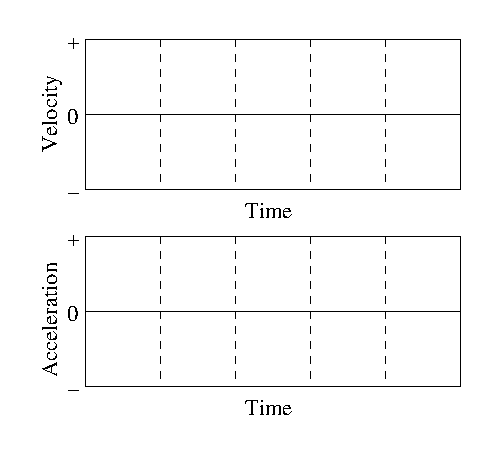
\includegraphics{slowing/slowing_fig15.eps} \par}
\vspace{1.3cm}

12. The car starts from rest and moves toward the origin, speeding up at a steady
rate.

\vspace{0.3cm}
{\par\centering 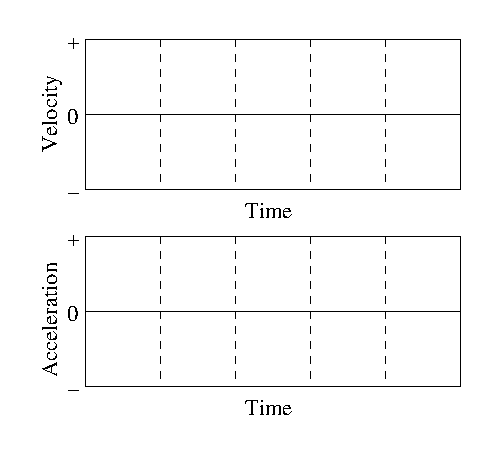
\includegraphics{slowing/slowing_fig15.eps} \par}
\vspace{1.3cm}

13. A ball is tossed in the air. It moves upward, reaches its highest point
and falls back downward. Sketch a velocity-time and an acceleration-time graph
for the ball from the moment it leaves the thrower's hand until the moment just
before it reaches her hand again. Consider the positive direction to be upward.

\vspace{0.3cm}
{\par\centering 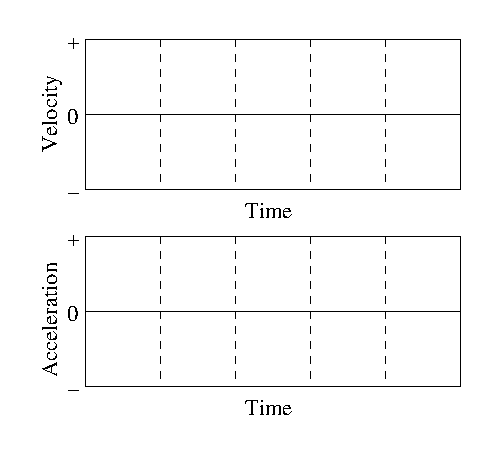
\includegraphics{slowing/slowing_fig15.eps} \par}
\vspace{0.3cm}

14. Each of the pictures below represents a car driving down a road. The motion
of the car is described. In each case, draw velocity and acceleration vectors
above the car which might represent the described motion. Also specify the sign
of the velocity and the sign of the acceleration. (The positive direction is toward the right.)

\newpage

(a) The driver has stepped on the accelerator and the car is just starting to
move forward.

\vspace{0.3cm}
{\par\centering 
\includegraphics{slowing/slowing_fig16.eps} \par}
\vspace{0.3cm}

(b) The car is moving forward. The brakes have been applied. The car is slowing
down, but has not yet come to rest.

\vspace{0.3cm}
{\par\centering 
\includegraphics{slowing/slowing_fig16.eps} \par}
\vspace{0.3cm}

(c) The car is moving backward. The brakes have been applied. The car is slowing down, but has not yet come to rest.

\vspace{0.3cm}
{\par\centering 
\includegraphics{slowing/slowing_fig16.eps} \par}
\vspace{0.3cm}

The following graphs represent the motions of objects along the positive position axis. Notice that the motion of the objects is represented by position, velocity, or acceleration graphs.

Answer the following questions. You may use a graph more than once or not at
all, and there may be more correct choices than blanks. If none of the graphs
is correct, answer none.

\vspace{0.3cm}
{\par\centering 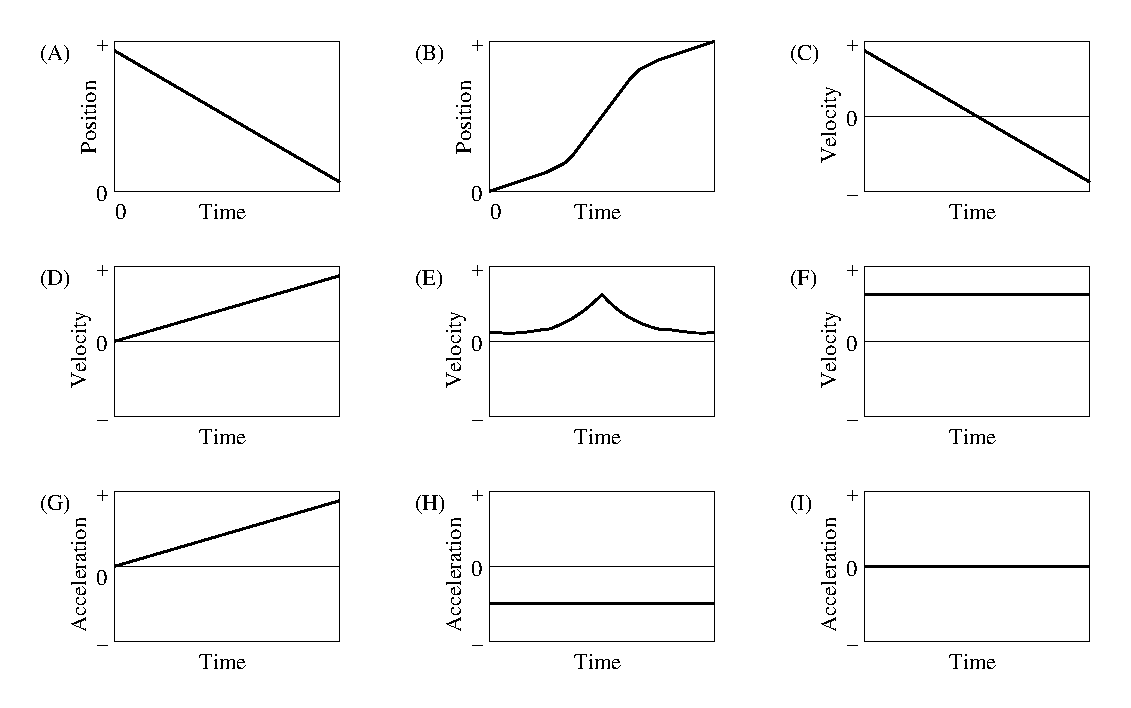
\includegraphics[width=6.5in]{slowing/slowing_fig17.eps} \par}
\vspace{0.3cm}

15. Pick one graph that gives enough information to indicate that the velocity
is always negative. \rule{0.5in}{0.1pt}

Pick three graphs that represent the motion of an object whose velocity is constant.

16. \rule{0.5in}{0.1pt} 17. \rule{0.5in}{0.1pt} 18. \rule{0.5in}{0.1pt}

19. Pick one graph that definitely indicates an object has reversed direction.
\rule{0.5in}{0.1pt}

20. Pick one graph that might possibly be that of an object standing still.
\rule{0.5in}{0.1pt}

Pick 3 graphs that represent the motion of objects whose acceleration is changing.

21. \rule{0.5in}{0.1pt} 22. \rule{0.5in}{0.1pt} 23. \rule{0.5in}{0.1pt}

Pick a velocity graph and an acceleration graph that could describe the motion
of the same object during the time shown.

24. Velocity graph. \rule{0.5in}{0.1pt} 25. Acceleration graph. \rule{0.5in}{0.1pt}



\setcounter{activity}{0}

\section{Projectile Motion\footnote{
1990-93 Dept. of Physics and Astronomy, Dickinson College. Supported by FIPSE
(U.S. Dept. of Ed.) and NSF. Portions of this material have been modified locally
and may not have been classroom tested at Dickinson College.
}}

Name \rule{2.0in}{0.1pt}\hfill{}Section \rule{1.0in}{0.1pt}\hfill{}Date \rule{1.0in}{0.1pt}

\textbf{Objectives }

To understand the experimental and theoretical basis for describing projectile
motion as the superposition of two independent motions: (1) a body falling in
the vertical direction, and (2) a body moving in the horizontal direction with
no forces.

\textbf{Apparatus}

\begin{itemize}
\item A tennis ball. 
\item A movie scaling ruler.
\item A video analysis system (\textit{Tracker}). 
\item Graphing and curve fitting software (\textit{Excel}).
\end{itemize}
\textbf{Activity \stepcounter{activity}\arabic{activity}: Predicting the Two-Dimensional Motion of a Tossed Ball }

\begin{enumerate}

\item Toss a tennis ball up at an angle of about 60\( ^{\circ } \) with the horizontal
a couple of times. Sketch the motion and describe it in words below. What is
the shape of the trajectory?
\vspace{20mm}

\item Let's consider the horizontal and vertical components of the motion separately.
What do you think is the horizontal motion of the ball? Is it motion with constant
velocity, constant acceleration, or some other kind of motion? (Hint: What
is the force acting on the ball in the horizontal direction after it is released?)
\vspace{20mm}

\item What do you think is the vertical motion of the ball? Is it motion with
constant velocity, constant acceleration, or some other kind of motion?
(Hint: What is the force acting on the ball in the vertical direction after
it is released?)
\vspace{20mm}

\end{enumerate}

The two-dimensional motion of a tossed ball is too fast to observe carefully
by eye without the aid of special instruments. In the next activity we will
use a video analysis system to study the motion of a small ball launched at
an angle of about 60\( ^{\circ } \) with respect to the horizontal. You are
to use the video analysis software and mathematical modeling techniques to find
the equations that describe: (a) the trajectory ($y$ vs. $x$), 
(b) the horizontal
motion ($x$ vs. $t$), and (c) the vertical motion ($y$ vs. 
$t$) of the projectile.

\newpage

\textbf{Activity \stepcounter{activity}\arabic{activity}: Analyzing Projectile Motion} 

\begin{enumerate}

\item Make a movie of a tennis ball in flight by following these steps. 

\begin{enumerate}
\item Set up the video camera and center the field of view on the region where you
will toss the ball. This region should be about 2 meters from the camera to
get a large enough area for the flight of the ball. Place a ruler or meter stick
somewhere in the field of view close to the plane of the motion of the ball
where it won't interfere with the motion. This ruler will be used later to determine
the scale. 
\item Make a movie of the tennis ball flying through the air with a significant component
of its initial velocity in the horizontal direction (i.e., don't toss it straight
up). Make sure most of the complete trajectory is visible to the camera. See
\textbf{Appendix D: Video Analysis} for details on making the movie. 
%When you
%save the movie file give it the name \textit{Projectile}.

\end{enumerate}

\item Determine the position of the projectile at different times during the motion.
To do this task follow the instructions in \textbf{Appendix
D: Video Analysis} for recording and calibrating the position data. When you
are analyzing the movie place the origin at the position of the ball in your
first frame. 
When you have finished marking the ball's position, export the data into
an \textit{Excel} file as described in \textbf{Appendix D}.

\item  Open your data in \textit{Excel}.
Launch \textit{Excel}. 
See \textbf{Appendix C: Introduction to Excel} for details on using
\textit{Excel}. Make a plot of the vertical position ($y$) versus the
horizontal position ($x$). Determine the equation that describes the trajectory
of the projectile. When you have found a good fit to the data, print the graph
and attach a copy to this unit. Write the equation for the trajectory of the
projectile in the space below. What is the shape of the trajectory? Does the
result agree with your earlier prediction?
\vspace{20mm}

\item Determine the equation that describes the horizontal motion of the projectile
by plotting the horizontal position ($x$) versus time ($t$) using 
\textit{Excel} using a polynomial fit.
Find a good fit to the data with \textit{Excel}. When you have
found a good fit to the data, print the graph and attach a copy to this unit.
What kind of motion is it? Does the result agree with your earlier prediction?
\textbf{Note:} Numbers from your graph should be rounded off to no more than three significant figures.
\vspace{6mm}

\begin{enumerate}
\item The equation for the horizontal component of the motion with proper units is:
$x =$\vspace{5mm}

\item The horizontal component of the acceleration with proper sign and units is:
\( a_{x}= \) \vspace{5mm}

\item The horizontal component of the initial velocity with proper sign and units
is: \( v_{0x}= \)\vspace{5mm}

\item The initial $x$ position with proper units is: \( x_{0}= \)\vspace{5mm}

\end{enumerate}

\item Determine the equation that describes the vertical motion of the projectile
by plotting the vertical position ($y$) versus time ($t$). Find a good fit to the
data using a polynomial.  When you have found a good fit to the data, print the graph and attach
a copy to this unit. What kind of motion is it? Does the result agree with your
earlier prediction?
\vspace{20mm}

\begin{enumerate}
\item The equation for the vertical component of the motion with proper units is:
$y =$\vspace{5mm}

\item The vertical component of the acceleration with proper sign and units is: 
\( a_{y}= \)
\vspace{5mm}

\item The vertical component of the initial velocity with proper sign and units is:
\( v_{0y}= \) \vspace{5mm}

\item The initial $y$ position with proper units is: \( y_{0} =\) \vspace{5mm}

\end{enumerate}

\item Does it appear that projectile motion is simply the superposition of two
types of motion that we have already studied? Explain.
\vspace{20mm}

\item Go around to the other groups in the lab and ask them for their measured values of the horizontal and vertical accelerations.
Make a histogram of your results for each component and calculate the average and standard deviation of each one.
For information on making histograms, see \textbf{Appendix C}. For information on calculating the average and
standard deviation, see \textbf{Appendix A}. Record the average and standard deviation here.
Attach the histogram to the unit.
\vspace{20mm}

\item What is your expectation for the vertical acceleration of the ball? Is your data consistent with your expectation?
Is the acceleration the same for the entire class? 
Use the average and standard deviation for the class to quantitatively answer these questions.
\vspace{20mm}

\item What is your expectation for the horizontal acceleration of the ball?  Is your data consistent with your expectation?
\vspace{20mm}

\item What does the histogram of the class data for the vertical component of the acceleration tell you? Be quantitative in your answer.
\vspace{20mm}

\end{enumerate}



\setcounter{activity}{0}

\section{Force and Motion\footnote{
1990-93 Dept. of Physics and Astronomy, Dickinson College. Supported by FIPSE
(U.S. Dept. of Ed.) and NSF. Portions of this material may have been modified
locally and may not have been classroom tested at Dickinson College.
}}

Name \rule{2.0in}{0.1pt}\hfill{}Section \rule{1.0in}{0.1pt}\hfill{}Date \rule{1.0in}{0.1pt}

\textbf{Objectives }

\begin{itemize}
\item To learn how to use a force probe to measure force. 
\item To understand the relationship between forces applied to an object and its motions. 
\item To find mathematical relationships among the force applied to an object, its acceleration, and the directions of the force and acceleration.
\end{itemize}

\textbf{Overview }

In the previous labs, you have used a motion detector to display position-time,
velocity-time and acceleration-time graphs of the motion of different objects.
You were not concerned about how you got the objects to move, i.e., what forces
(pushes or pulls) acted on the objects. From your experiences, you know that
force and motion are related in some way. To start your bicycle moving, you
must apply a force to the pedal. To start up your car, you must step on the
gas pedal to get the engine to apply a force to the road through the tires.

But, exactly how is force related to the quantities you used in the previous
unit to describe motion --- position, velocity and acceleration? In this unit you
will pay attention to forces and how they affect motion. You will apply forces
to a cart, and observe the nature of its resulting motion graphically with a
motion detector.


\textbf{Apparatus} 

\begin{itemize}
\item \textit{Science Workshop 750 Interface}
\item Force probe 
\item Variety of hanging masses 
\item Low friction pulley and string 
\item Motion detector 
\item Dynamics cart (with flag) and track 
\item \textit{DataStudio} software (V, A \& F Graphs application)
\end{itemize}

\textbf{Measuring Forces} 

In this investigation you will use a force probe (also called a force sensor) to measure forces. 
The force probe puts out a voltage signal proportional to the force applied to the arm of the probe. 
Physicists have defined a standard unit of force called the newton, abbreviated N. 
For your work on forces and the motions they cause, it will be more convenient to have the force 
probe read directly in newtons rather than voltage
so the force probe must be calibrated. 
To calibrate the force probe, see \textit{Calibrating Force Sensors} in \textbf{Appendix E: Instrumentation}.

\textbf{Motion and Force} 

Now you can use the force probe to apply measured amounts of force to an object.
You can also use the motion detector, as in the previous units, to examine the
motion of the object. In this way you will be able to establish the relationship
between motion and force.
\vspace{10mm}

\newpage

\textbf{Activity \stepcounter{activity}\arabic{activity}: Pushing and Pulling a Cart} 

In this activity you will move a cart by pushing and pulling it with your hand.
You will measure the force, velocity and acceleration. Then you will be able
to look for relationships between the applied force and the motion quantities.

\begin{enumerate}

\item Calibrate the force probe if you haven't already done so (see \textit{Calibrating Force Sensors} 
in \textbf{Appendix E: Instrumentation}). 
Then set up the cart, force probe and motion detector on the level track as shown in Figure \ref{forcefig1}. 
Measure and record the mass of the cart and force probe assembly (using the compact scale).

\vspace{10mm}

\begin{figure}[hbt]
\begin{center}
{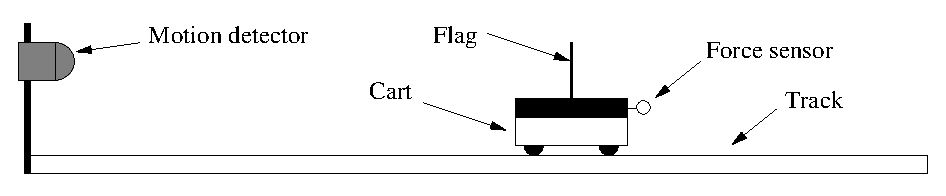
\includegraphics{iqsForce/force1_fig1b.eps}}
\caption{Equipment setup for qualitative measurements of force and motion.}\label{forcefig1}
\end{center}
\end{figure}


\item Suppose you grasp the hook on the force probe and move the cart forwards
and backwards in front of the motion detector. Do you think that either the
velocity or the acceleration graph will look like the force graph? Is either
of these motion quantities related to force? That is to say, if you apply a
changing force to the cart, will the velocity or acceleration change in the
same way as the force?
\vspace{30mm}

\item To test your predictions, open the V, A \& F Graphs application. Grasp the
hook on the force probe and start acquiring data. When you hear the clicks,
pull the cart away from the motion detector, and smoothly stop it. Then push
it back towards the motion detector, and again smoothly stop it. Be sure that
the cart never gets closer than 0.15 m away from the detector and be careful
of the wires. Repeat until you get a good run, and adjust 
the scale of the axes if necessary. Sketch your graphs on the axes below.

\vspace{0.3cm}
\begin{figure}[hbt]
\begin{center}
{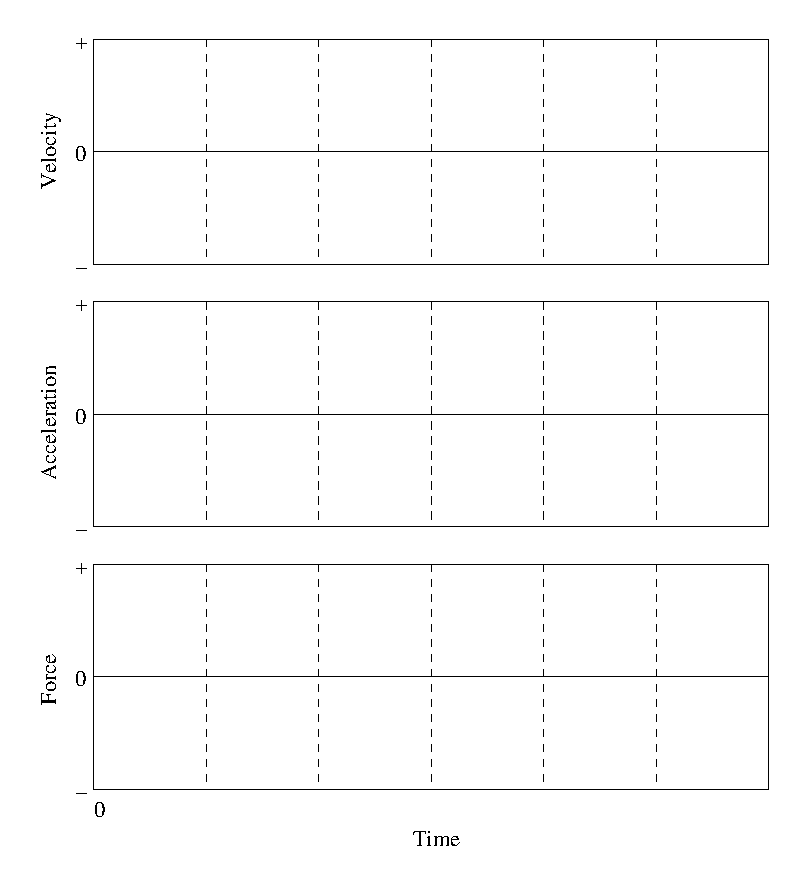
\includegraphics[width=4.4in]{iqsForce/force1_fig2.eps}}
\caption{Velocity, acceleration, and force versus time plots.}
\end{center}
\end{figure}
\vspace{0.3cm}

\item Does either graph--velocity or acceleration--resemble the force graph? Which
one? Explain.
\vspace{20mm}

\item Based on your observations, does it appear that either the velocity or acceleration
of the cart might be related to the applied force? Explain.
\vspace{20mm}

\end{enumerate}

%\newpage

\textbf{Activity \stepcounter{activity}\arabic{activity}: Finding the Relationship Between Acceleration and Force}

\begin{enumerate}

\item Use the {\it SmartTool} in {\it DataStudio} (see {\bf Appendix B: Introduction to DataStudio}) to record twelve or
so sets of acceleration ($a$) and force ($F$) values and enter them in the table below.

\begin{center}
\begin{table}[hbt]
\begin{center}
\begin{tabular}{|c|c|c|c|c|c|}\hline
Trial & $\qquad a(m/s^2)\qquad$ & $\qquad F(N)\qquad$ & Trial & $\qquad a(m/s^2)\qquad$ & $\qquad F(N)\qquad$ \\ \hline
1     &                         &                     & 7     &                         &                     \\ \hline
2     &                         &                     & 8     &                         &                     \\ \hline
3     &                         &                     & 9     &                         &                     \\ \hline
4     &                         &                     & 10    &                         &                     \\ \hline
5     &                         &                     & 11    &                         &                     \\ \hline
6     &                         &                     & 12    &                         &                     \\ \hline
\end{tabular}
\caption{Measured values of force and acceleration.}
\end{center}
\end{table}
\end{center}

\newpage

\item Make a plot of force versus acceleration with properly labeled axes with units.
Attach it to this unit.
Are force and acceleration proportional to each other? Why or why not?

\vspace{15mm}

\item If force is proportional to acceleration, then what is the value of the constant of 
proportionality (Hint: fit your data)?
What are its units? 

\vspace{15mm}

\item What is the equation that relates the force and the acceleration, 

\vspace{15mm}

\item How does the mass of your cart compare with the constant of 
proportionality between force and acceleration?
What does this say about the meaning of the constant of proportionality? About the meaning of mass?

\vspace{15mm}

\item Go around to the other groups in the lab and ask them for their measured values of the
constant of proportionality.
Check that the mass of their cart measured with the scale is similar to yours.
Make a histogram of the results and calculate the average and standard deviation.
For information on making histograms, see \textbf{Appendix C}. For information on calculating the average and
standard deviation, see \textbf{Appendix A}. Record the average and standard deviation here.
Attach the histogram to the unit.

\vspace{15mm}

\item Are the class results for the constant of proportionality consistent with the values from the scale?
Be quantitative in your answer.

\vspace{15mm}

\end{enumerate}

\newpage 

\textbf{Homework} 

\begin{enumerate}

\item A force is applied which makes an object move with the acceleration shown
below. Assuming that friction is negligible, sketch a force-time graph of the
force on the object on the axes below. Explain your answer.

\vspace{1.3cm}
{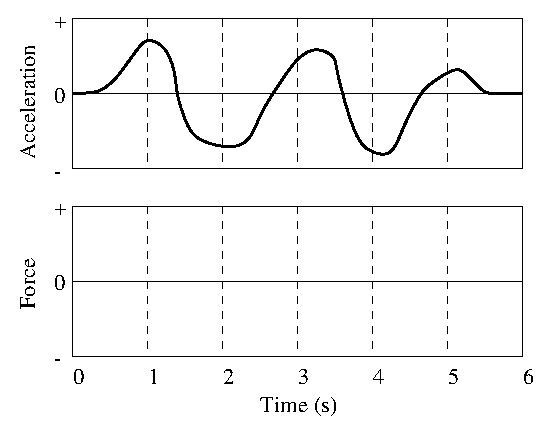
\includegraphics{iqsForce/force1_fig6.eps}}
\vspace{0.3cm}

\item Roughly sketch the velocity-time graph for the object in question 1 on the
axes below, beginning with a $negative$ velocity.

\vspace{0.3cm}
{\par\centering \includegraphics{iqsForce/force1_fig7.eps} \par}
\vspace{0.8cm}

\item A cart can move along a horizontal line (the + position axis). It moves with
the velocity shown below.

\vspace{0.3cm}
{\par\centering \includegraphics{iqsForce/force1_fig8.eps} \par}
\vspace{0.8cm}

Assuming that friction is so small that it can be neglected, sketch on the axes
that follow the acceleration-time and force-time graphs of the cart's motion.

\vspace{0.3cm}
{\par\centering \includegraphics{iqsForce/force1_fig9.eps} \par}
\vspace{0.3cm}

Explain both of your graphs.
\vspace{20mm}

\item The next three questions refer to an object which can move in either direction along a
horizontal line (the + position axis). Assume that friction is so small that
it can be neglected. Sketch the shape of the graph of the force applied to the
object which would produce the motion described. 

The object moves away from the origin with a constant acceleration.

\vspace{0.3cm}
{\par\centering \includegraphics{iqsForce/force1_fig10.eps} \par}
\vspace{0.3cm}

\item The object moves toward the origin with a constant acceleration.

\vspace{0.3cm}
{\par\centering \includegraphics{iqsForce/force1_fig10.eps} \par}
\vspace{0.3cm}

\newpage

\item The object moves away from the origin with a constant velocity.

\vspace{0.3cm}
{\par\centering \includegraphics{iqsForce/force1_fig10.eps} \par}
\vspace{0.3cm}

\noindent The next two questions refer to an object which can move along a horizontal line
(the + position axis). Assume that friction is so small that it can be ignored.
The object's velocity-time graph is shown below.

\vspace{0.3cm}
{\par\centering \includegraphics{iqsForce/force1_fig11.eps} \par}
\vspace{0.3cm}

\item Sketch the shapes of the acceleration-time and force-time graphs on the axes
below.

\vspace{0.3cm}
{\par\centering \includegraphics{iqsForce/force1_fig9.eps} \par}
\vspace{0.3cm}

\newpage

\item Suppose that the force applied to the object were twice as large. Sketch
with dashed lines on the same axes above the force, acceleration, and velocity.

The next question refers to an object which can move along a horizontal line (the +
position axis). Assume that friction is so small that it can be ignored. The
object's velocity-time graph is shown below.

\vspace{0.3cm}
{\par\centering \includegraphics{iqsForce/force1_fig12.eps} \par}
\vspace{0.3cm}

\item Sketch the shapes of the acceleration and force graphs on the axes below.

\vspace{0.3cm}
{\par\centering \includegraphics{iqsForce/force1_fig9.eps} \par}
\vspace{0.3cm}

\begin{comment}

The next five questions refer to a toy car which can move in either direction along a
horizontal line (the + position axis).

\vspace{0.3cm}
{\par\centering \includegraphics{iqsForce/force2_fig6.eps} \par}
\vspace{0.3cm}

Assume that friction is so small that it can be ignored. Sketch the shape of
the graph of the applied force which would keep the car moving as described
in each statement.

\item The toy car moves away from the origin with a constant velocity.

\vspace{0.3cm}
{\par\centering \includegraphics{iqsForce/force2_fig7.eps} \par}
\vspace{0.3cm}

\item The toy car moves away from the origin with a steadily decreasing velocity
(a constant acceleration).

\vspace{0.3cm}
{\par\centering \includegraphics{iqsForce/force2_fig7.eps} \par}
\vspace{0.3cm}

\item The toy car moves away from the origin, speeds up and then slows down.

\vspace{0.3cm}
{\par\centering \includegraphics{iqsForce/force2_fig7.eps} \par}
\vspace{0.3cm}

\item The toy car moves toward the origin with a steadily increasing speed ( a
constant acceleration).

\vspace{0.3cm}
{\par\centering \includegraphics{iqsForce/force2_fig7.eps} \par}
\vspace{0.3cm}

\item The toy car is given a push away form the origin and released. It continues
to move with a constant velocity. sketch the force after the car is released.

\vspace{0.3cm}
{\par\centering \includegraphics{iqsForce/force2_fig7.eps} \par}
\vspace{1.3cm}

\item A cart is moving toward the right and slowing down, as shown in the diagrams
below. Draw arrows above the cart representing the magnitudes and directions
of the net (combined) forces you think are needed on the cart at $t = 0$ s, 
$t
= 1$ s, etc. to maintain its motion with a steadily decreasing velocity.

\vspace{0.3cm}
{\par\centering \includegraphics{iqsForce/force2_fig9.eps} \par}
\vspace{0.3cm}

Explain the reasons for your answers.
\vspace{30mm}

\item If the positive direction is toward the right, what is the sign of the force
at $t = 2$ sec in question 9? Explain.
\vspace{30mm}

\end{comment}

\end{enumerate}


\setcounter{activity}{0}
\section{Centripetal Force\footnote{
1990-93 Dept. of Physics and Astronomy, Dickinson College. Supported by FIPSE
(U.S. Dept. of Ed.) and NSF. Portions of this material have been modified locally
and may not have been classroom tested at Dickinson College.
}}

Name \rule{2.0in}{0.1pt}\hfill{}Section \rule{1.0in}{0.1pt}\hfill{}Date \rule{1.0in}{0.1pt}

\textbf{Objective} 

To explore the phenomenon of uniform circular motion and the accelerations and
forces needed to maintain it.

\textbf{Overview} 

In a previous unit you began the study 
projectile motion. In this unit we are going to consider the application of
Newton's laws to another phenomenon in two dimensions. Since Newton's laws can
be used to predict types of motion or the conditions for no motion, their applications
are useful in many endeavors including human body motion, astrophysics, and
engineering.

You will explore uniform circular motion, in which an object moves at a constant
speed in a circle. In particular, you will develop a mathematical description
of centripetal acceleration and the force needed to keep an object moving in
a circle.

\vspace{0.3cm}
{\par\centering \includegraphics{iqsCentripetalForce/centripetal_fig1b.eps} \par}
\vspace{0.3cm}

\textbf{Apparatus}

\begin{itemize}
\item An airplane. 
\item A video analysis system ({\it Tracker}). 
\item {\it DataStudio}
\item A ruler. 
\item Graphing software ({\it Excel}). 
\end{itemize}
\textbf{Moving in a Circle at a Constant Speed }

When a race car speeds around a circular track, or when David twirled a stone
at the end of a rope to clobber Goliath, or when a planet like Venus orbits
the sun, they undergo uniform circular motion. Understanding the forces which
govern orbital motion has been vital to astronomers in their quest to understand
the laws of gravitation. 

But we are getting ahead of ourselves, for as we have done in the case of linear
and projectile motion we will begin our study by considering situations involving
external applied forces that lead to circular motion in the absence of friction.

\vspace{0.3cm}
{\par\centering \includegraphics{iqsCentripetalForce/centripetal_fig2b.eps} \par}
\vspace{0.3cm}

Let's begin our study with some very simple considerations. Suppose an astronaut
goes into outer space, ties a ball to the end of a rope, and spins the ball
so that it moves at a constant speed.

\textbf{Activity \stepcounter{activity}\arabic{activity}: Uniform Circular Motion }

\begin{enumerate}

\item Consider the figure above. What is the speed of a ball that moves in a circle
of radius $r = 2.5$ m if it takes 0.50 s to complete one revolution?
\vspace{20mm}

\item The speed of the ball is constant! Would you say that this is accelerated
motion?
\vspace{20mm}

\item What is the definition of acceleration? (Remember that acceleration is a
vector!)
\vspace{20mm}

\item Are velocity and speed the same thing? Is the velocity of the ball constant?
(Hint: Velocity is a vector quantity!)
\vspace{20mm}

\item In light of your answers to (c) and (d), would you like to change your answer
to part (b)? Explain.
\vspace{20mm}

\end{enumerate}

\textbf{Using Vectors to Diagram How Velocity Changes} 

By now you should have concluded that since the direction of the motion of an
object undergoing uniform circular motion is constantly changing, its velocity
is also changing and thus it is accelerating. We would like you to figure out
how to calculate the direction of the acceleration and its magnitude as a function
of the speed $v$ of an object such as a ball as it revolves and as a function
of the radius of the circle in which it revolves. In order to use vectors to
find the direction of velocity change in circular motion, let's review some
rules for adding velocity vectors.

\vspace{0.3cm}
{\par\centering \includegraphics{iqsCentripetalForce/circ_motion_fig1b.eps} \par}
\vspace{0.3cm}

\begin{enumerate}
\item To Draw Velocities: Draw an arrow representing the velocity, \( 
{\bf v}_{1} \), of
the object at time \( t_{1} \). Draw another arrow representing the velocity,
\( {\bf v}_{2} \), of the object at time \( t_{2} \). 
\item To Draw Velocity Change: Find the change in the velocity 
\( \Delta  {\bf v}
= {\bf v}_{2}  - {\bf v}_{1} \) during the time interval described
by \( \Delta  t = t_{2}  - t_{1} \). Start by using the rules of
vector sums to rearrange the terms so that \({\bf v}_{1}  +  \Delta  
{\bf v}
= {\bf v}_{2} \). Next place the tails of the two velocity vectors together
halfway between the original and final location of the object. The change in
velocity is the vector that points from the head of the first velocity vector
to the head of the second velocity vector. 
\item To Draw Acceleration: The acceleration equals the velocity change 
\( \Delta  {\bf v}\)
divided by the time interval $t$ needed for the change. Thus, \textbf{a} is in
the same direction as \( \Delta  {\bf v}\) but is a different length (unless
\( \Delta  t = 1\)). Thus, even if you do not know the time interval, you
can still determine the direction of the acceleration because it points in the
same direction as \( \Delta  {\bf v}\). 
\end{enumerate}
The acceleration associated with uniform circular motion is known as centripetal
acceleration. You will use the vector diagram technique described above to find
its direction. 

\textbf{Activity \stepcounter{activity}\arabic{activity}: The Direction of Centripetal Acceleration }

\begin{enumerate}

\item Determine the direction of motion of the ball shown below if it is moving
counter-clockwise at a constant speed. Note that the direction of the ball's
velocity is always tangential to the circle as it moves around. Draw an arrow
representing the direction and magnitude of the ball's velocity as it passes
the dot just before it reaches point A. Label this vector \textbf{v}\( _{1} \). 

\vspace{0.3cm}
{\par\centering \includegraphics{iqsCentripetalForce/circ_motion_fig2b.eps} \par}
\vspace{0.3cm}

\item Next, use the same diagram to draw the arrow representing the velocity of
the ball when it is at the dot just after it passes point A. Label this vector
\textbf{v}\( _{2} \).

\item Find the direction and magnitude of the change in velocity as follows. In
the space below, make an exact copy of both vectors, placing the tails of the
two vectors together. Next, draw the vector that must be added to vector \textbf{v}\( _{1} \)
to add up to vector \textbf{v}\( _{2} \) ; label this vector \( \Delta  \)\textbf{v}.
Be sure that vectors \textbf{v}\( _{1} \) and \textbf{v}\( _{2} \) have the
same magnitude and direction in this drawing that they had in your drawing in
part (a)!
\vspace{30mm}

\item Now, draw an exact copy of \( \Delta  \)\textbf{v} on your sketch in part
(a). Place the tail of this copy at point A. Again, make sure that your copy
has the exact magnitude and direction as the original \( \Delta  \)\textbf{v}
in part (c).
\vspace{30mm}

\item Now that you know the direction of the change in velocity, what is the direction
of the centripetal acceleration, \textbf{a}\( _{c} \)?
\vspace{18mm}

\item If you did the same analysis for point B at the opposite end of the circle,
what do you think the direction of the centripetal acceleration, \textbf{a}\( _{c} \),
would be now?
\vspace{18mm}

\item As the ball moves on around the circle, what is the direction of its acceleration?
\vspace{18mm}

\item Use Newton's second law in vector form (\( \sum {\bf F} = m{\bf a}\)
) to describe the direction of the net force on the ball as it moves around
the circle.
\vspace{18mm}

\item If the ball is being twirled around on a string, what is the source of the
net force needed to keep it moving in a circle?
\vspace{18mm}

\end{enumerate}

\newpage 

\textbf{Using Mathematics to Derive How Centripetal Acceleration Depends on
Radius and Speed }

You haven't done any experiments yet to see how centripetal acceleration depends
on the radius of the circle and the speed of the object. You can use the rules
of mathematics and the definition of acceleration to derive the relationship
between speed, radius, and magnitude of centripetal acceleration. 

\textbf{Activity \stepcounter{activity}\arabic{activity}: How Does a\( _{c} \) Depend on v and r?} 

\begin{enumerate}

\item Do you expect you would need more centripetal acceleration or less centripetal
acceleration to cause an object moving at a certain speed to rotate in a smaller
circle? In other words, would the magnitude, a\( _{c} \), have to increase
or decrease as r decreases if circular motion is to be maintained? Explain.
\vspace{20mm}

\item Do you expect you would need more centripetal acceleration or less centripetal
acceleration to cause an object to rotate at a given radius $r$ if the speed $v$
is increased? In other words, would the magnitude, \( a_{c} \), have to increase
or decrease as $v$ increases if circular motion is to be maintained? Explain.
\vspace{20mm}

\end{enumerate}

You should have guessed that it requires more acceleration to move an object
of a certain speed in a circle of smaller radius and that it also takes more
acceleration to move an object that has a higher speed in a circle of a given
radius. Lets use the definition of acceleration in two dimensions and some accepted
mathematical relationships to show that the magnitude of centripetal acceleration
should actually be given by the equation
\begin{equation}
a_{c}=\frac{v^{2}}{r}
\end{equation}

In order to do this derivation you will want to use the following definition
for acceleration
\begin{equation}
\left\langle {\bf a}\right\rangle =\frac{{{\bf v}_{2}}-{{\bf v}_{1}}}{t_{2}-t_{1}}=\frac{\Delta {\bf v}}{\Delta t}
\end{equation}

\textbf{Activity \stepcounter{activity}\arabic{activity}: Finding the Equation for a\( _{c} \) }

\begin{enumerate}

\item Refer to the diagram below. Explain why, at the two points shown on the
circle, the angle between the position vectors at times \( t_{1} \) and \( t_{2} \)
is the same as the angle between the velocity vectors at times \( t_{1} \)
and \( t_{2} \). Hint: In circular motion, velocity vectors are always perpendicular
to their position vectors.

\vspace{0.3cm}
{\par\raggedright \hspace{0.1in}\includegraphics[height=2.0in]{iqsCentripetalForce/centripetal5c.eps}\put(20,30){\includegraphics[height=1.0in]{iqsCentripetalForce/centripetal8h.eps}} \par}
\vspace{0.3cm}

\item Since the angles are the same and since the magnitudes of the displacements
never change (i.e., \(r= r_{1}  = r_{2} \)) and the magnitudes of the
velocities never change (i.e., \(v = v_{1}  = v_{2} \)), use the properties
of similar triangles to explain why \( \frac{\Delta v}{v}=\frac{\Delta r}{r} \).\label{simtri}
\vspace{20mm}

\item Now use the equation in part \ref{simtri} and the definition of 
$\langle a \rangle$ to show that
\( \left\langle a_{c}\right\rangle =\frac{\Delta v}{\Delta t}=\frac{\left( \Delta r\right) }{\left( \Delta t\right) }\frac{v}{r}. \)\label{aveac}
\vspace{20mm}

\item The speed of the object as it rotates around the circle is given by \( v=\frac{\Delta s}{\Delta t} \).
Is the change in arc length, \( \Delta s \), larger or smaller than the magnitude
of the change in the position vector, \( \Delta r \)? Explain why the arc length
change and the change in the position vector are approximately the same when
$t$ is very small (so that the angle $\theta$ becomes very small) i.e., why is
\( \Delta  s
 \simeq   \Delta  r\)?
\vspace{20mm}

\item If \( \Delta s  \simeq   \Delta  r\), then what is the equation
for the speed in terms of \( \Delta  r\) and \( \Delta  t\)?
\vspace{20mm}

\item Using the equation in part \ref{aveac} above, show that as \( \Delta t  \rightarrow 0 \),
the instantaneous value of the centripetal acceleration is given by Eq. 1.
\vspace{20mm}

\item If the object has a mass $m$, what is the equation for the magnitude of the
centripetal force needed to keep the object rotating in a circle (in terms of
$v$, $r$, and $m$)? In what direction does this force point as the object rotates
in its circular orbit?
\vspace{20mm}

\end{enumerate}

\textbf{Experimental Test of the Centripetal Force Equation }

The theoretical considerations in the last activity should have led you to the
conclusion that, whenever you see an object of mass $m$ moving in a circle of
radius $r$ at a constant speed $v$, it must at all times be experiencing a net centripetal
force directed toward the center of the circle that has a magnitude of
\begin{equation}
F_{c}=ma_{c}=m\frac{v^{2}}{r}\label{eq:Fcent}
\end{equation}

Let's check this out. Does this rather odd equation really work for an external
force?

To test the validity of the derivation we must compare it to experience. We
will use a ``toy'' airplane suspended from a string and flying
in a circular path. See Figure \ref{fig:airplane}. 
We will use the video analysis system to measure the properties
of the motion and determine the horizontal and vertical components of the force
exerted on the airplane using Equation \ref{eq:Fcent}. We will compare that result with a
direct measurement of the tension in the string using a force sensor. 
\begin{figure}
\begin{center}
\includegraphics[height=4.0in]{iqsCentripetalForce/airplaneSetupB.eps}
\caption{Setup for testing the centripetal force equation. Red line is the
string from the force sensor to the airplane.}\label{fig:airplane}
\end{center}
\end{figure}

\textbf{Activity \stepcounter{activity}\arabic{activity}: Verifying the F\( _{c} \) Equation }

\begin{enumerate}

\item To test the validity of Equation \ref{eq:Fcent} you will analyze data that has already been collected
(because of time constraints).
Download the movie {\it airplaneMovie.wmv} from the location\raggedright

{\verb!https://facultystaff.richmond.edu/~ggilfoyl/genphys/131/links.html!}

\noindent and store it on your computer {\tt Desktop}.
Download the {\it DataStudio} file {\it airplaneData.ds} from the same site and also store it on your {\tt Desktop}.

\item Some of the parameters of the airplane's ``flight'' are
\[
m_{plane} = 0.172~kg \qquad l_{plane} = 0.169~m \qquad L = 0.984~m
\]
where $m_{plane}$ is the mass of the plane, $l_{plane}$ is the length of the plane, and $L$
is the distance from the center of mass of the airplane, along the string, up to the pivot where
the string becomes vertical. See Figure \ref{fig:airplane}.

\item Determine the force exerted by the string as shown in Figure \ref{fig:airplane}.
Open {\it DataStudio} (Go to {\tt Start $\rightarrow$ All Programs $\rightarrow$ Physics  Application $\rightarrow$ DataStudio} 
and click `Open Activity' on the pop-up window when {\it DataStudio} starts.
Open the file you just downloaded.
You will see a measurement of the force exerted by the string on the airplane as a function of time.
The measurement was made using a force sensor.
See Figure \ref{fig:airplane}.
A string was attached from the hook on the sensor (red line in Figure \ref{fig:airplane}), ran vertically downward, passed through 
a small hole in a fixed steel rod (the pivot), and then was attached to the airplane.
This setup allowed the string to rotate freely so the only forces acting on the airplane were
gravity and the tension in the string (the friction force here is very small).
There are two distinct regions on your plot; where the airplane was orbiting ($0 < t < 40~s$)and then after it was caught
and placed on the lab table so the tension in the string went to zero ($45~s < t < 65~s$).
Use the {\it DataStudio} tools to measure the average force exerted by the string while it was orbiting.
Record your answer here along with the standard deviation.\label{getFscale}\\
\vspace{2mm}

\hspace{0.5in} $F_{scale} = \qquad\qquad \pm$

\vspace{5mm}

\item Determine the position of the airplane during at least two complete revolutions. To
do this task follow the instructions in the second section of \textbf{Appendix D: Video Analysis} 
for analyzing a movie file with {\it Tracker}.
Calibrate your plot with the known length of the airplane $l_{plane}$.
When finished, you may want to export your measurements to a file for safekeeping.

\item Make a plot of all the points on the trajectory of the airplane during those two  revolutions  
by turning on all the measured points by clicking on {\bf Set trail length} (see {\bf Appendix D}).
Print your plot and attach it to your lab.

\item Is the motion circular? What is your evidence?
\vspace{10mm}

\item Use a ruler and your plot to measure the diameter of the airplane's trajectory.
Make at least five separate measurements between different diameters of the trajectory
and enter them in the table below.
Use the known length of the airplane $l_{plane}$ to convert those measurements to the scale of
the movie and then calculate each radius.

\begin{table}[h!]
\begin{center}
\begin{tabular}{|c|c|c|} \hline
Measured  &  Converted  &            \\
Diameter  &  Diameter   & Radius (m) \\ \hline
          &             &            \\
          &             &            \\
          &             &            \\
          &             &            \\
          &             &            \\
          &             &            \\
          &             &            \\ \hline
\end{tabular}
\end{center}
\end{table}

\item What is the average radius of the motion? \\
\vspace{2mm}

\hspace{0.5in} $r_{ave} =$

\vspace{5mm}

\item To test the validity of the expression for \( F_{c} \) we must know the
speed. Use the measurements of the radius of the airplane's trajectory and the
time for at least two complete revolutions to calculate the average speed.
The time is recorded in the data table in {\it Tracker}.
\vspace{5mm}

\hspace{0.5in} \( v_{ave} \) = 
\vspace{5mm}

\newpage

\item Use your results for the mass, the average velocity of the airplane, and
the average radius of the circular motion to calculate the centripetal force exerted by
the string.\label{getFc}
\vspace{5mm}

\hspace{0.5in} \( F_{c} \) = 
\vspace{5mm}

\item We will now determine the net force exerted by the string on the airplane
by using a little trigonometry.
Recall that we know $r_{ave}$, the radius of the airplane's circular path, and 
$L$, the total length of the string that is actually rotating. 

\begin{enumerate}
\item Using these two distances ($r_{ave}$ and $L$), 
calculate the angle the string makes with
the horizontal. You may want to draw a diagram to do this. \\
\vspace{5mm}

\( \theta  =\)  \vspace{5mm}

\item We determined the horizontal component of the force on the airplane 
\( F_{c} \) in part \ref{getFc}. Knowing the angle \( \theta \) we can determine an
expression for the
net force exerted by the string on the airplane, \( F_{plane} \). Draw a vector
force diagram including \( F_{c} \) and \( F_{plane} \), derive an expression
for \( F_{plane} \) and calculate it. \\
\vspace{5mm}

\( F_{plane} =\)  \vspace{30mm}

\end{enumerate}

\item Compare your result for \( F_{plane} \) with the measurement of the spring
scale \( F_{scale} \) from part \ref{getFscale}. Should they be different? Should they be the same? Explain.
\vspace{30mm}


\item Calculate the difference between \( F_{plane} \) and \( F_{scale} \) (\( F_{plane} - F_{scale} \))and record it below.
Go around to the other lab groups and get their results for this quantity.
Make a histogram of the results you collect and calculate the average and standard deviation.
Print the histogram and attach it to this unit.
For information on making histograms, see \textbf{Appendix C}. For information on calculating the average and
standard deviation, see \textbf{Appendix A}. Record the average and standard deviation here.
\vspace{30mm}

\newpage

\item What is your expectation for the difference \( F_{plane} - F_{scale} \)?
Do the data from the class support this expectation? 
Use the average and standard deviation for the class to quantitatively answer this question.
\vspace{15mm}

\item What does the histogram of the class data tell you? Be quantitative in your answer.
\vspace{15mm}

\item Discuss the major sources of uncertainty in this experiment.
\vspace{15mm}

\end{enumerate}


% appendices.

P7 332
#XVVERSION:version 3.10a-jumboFix+Enh of 20081216 (interim!)+FLmask
#BUILTIN:UNKNOWN
#IMGINFO:
#END_OF_COMMENTS


P7 332
#XVVERSION:version 3.10a-jumboFix+Enh of 20081216 (interim!)+FLmask
#BUILTIN:UNKNOWN
#IMGINFO:
#END_OF_COMMENTS


P7 332
#XVVERSION:version 3.10a-jumboFix+Enh of 20081216 (interim!)+FLmask
#BUILTIN:UNKNOWN
#IMGINFO:
#END_OF_COMMENTS



\section{Video Analysis}

\textbf{Making a Movie with ``Windows Live Movie Maker''} 

To make a movie, perform the following steps:

\begin{enumerate}

\item Make sure the camera is connected to a USB port on your computer. 
Close all windows, applications, programs, and browsers.

\item Click the {\bf Start} button in the lower-left corner of your screen and type `movie maker' in the Search programs and files box. 
Once the search results appear, click on {\bf Windows Live Movie Maker} under {\bf Programs}. 
After movie maker starts, close any pop-up windows that may appear.

\item Click the {\bf Webcam Video} button. 
A webcam video window opens. 
Enlarge the video frame by dragging the vertical line on the right side of the video frame.

\item Position the camera 2-3 meters from the object you will be viewing. 
Adjust the camera height and orientation so that the field of view is 
centered on the expected region where the object will move. 

\item Place a meter stick or an object of known size in the field of view where 
it won't interfere with the experiment. 
The meter stick should be the same distance away from the camera as the motion 
you are analyzing so the horizontal and vertical scales will be accurately determined. 
It should also be parallel to one of the sides of the movie frame. 
Make sure that the meter stick is not far away from the central region of field of view, and that it is perpendicular to the line of sight of camera.

\item One member of your group should perform the computer tasks while the other does the experiment.

\item To start recording your video, click {\bf Record}. When you are done, click {\bf Stop}. 

Save the video on your Desktop with a unique name that you can easily identify.
 The video will be saved in Windows Media Video format, i.e. with extension wmv. (Do not save the video as a Movie Maker Project file.)

\end{enumerate}

\textbf{Analyzing the Movie} 

To determine the position of an object at different times during the
motion, perform the following steps:

\begin{enumerate}

\item Start up Tracker by going to {\bf Start} $\rightarrow$ {\bf All Programs} $\rightarrow$ 
{\bf Physics Applications} $\rightarrow$ {\bf Tracker}. 
When {\bf Tracker} starts it appears as shown below. The menu icons and buttons that we will use are identified by arrows.
\begin{figure}[hbt]
\begin{center}
\includegraphics[width=5.5in]{appendices/video_analysis_tracker_fig1d.eps}
\caption{Initial {\bf Tracker} window for video analysis.}
\end{center}
\end{figure}

\item Click the {\bf Open Video} button on the toolbar (see figure below) to import your video. 
After your video is imported, Tracker will warn you that the video frames don't have the same time duration. 
This is okay since Windows Live Movie Maker uses a variable frame rate. 
Click {\bf Close} on the warning window to ignore Tracker's recommendation.

\item Click the {\bf Clip Settings} button (see figure below) to identify the frames you wish to analyze. 
A clip settings dialog box appears. 
Here, you only need to identify and set the start and end frames. 
Leave everything else in the dialog box unchanged. 
To find and set the start frame, drag the player's left slider to scan forward through the video, and 
stop when you get to the first frame of interest. 
Now, the start frame is set and the corresponding frame number should be displayed in the dialog box. 
If not, then click on the {\bf Start Frame} in the dialog box, enter the number of the frame 
(printed in the lower right part of the Tracker window), and click outside the box.
Then, click the {\bf Play video} button to go to the last frame in the video. 
Next, drag the player's right slider to scan backward through the video to find the last frame of interest. 
Stop when you get to the frame of interest. Now, the end frame is also set and the corresponding frame number should be displayed in the dialog box. 
If not, then click on the {\bf End Frame} in the dialog box, enter the number of the frame, and click outside the box.
Finally, click the {\bf OK} button to close the dialog box, and then click the player's {\bf Return} button to return to the start frame.

\item Click the {\bf Calibration} button (see the figure) and select the {\bf calibration stick}. 
A blue calibration line appears on the video frame. 
Drag the ends of this blue line to the ends of your calibration meter stick. 
Then click the readout box on the calibration line to select it. 
Enter the length of the meter stick in this box (without units). 
For example, if your calibration meter stick is 1.00 meter long, enter 1.00 in the box 
and then click outside the box to accept the value or hit {\bf Return}. 
At this point, you can right-click the video frame to zoom in for more accurate adjustment of the ends 
of the calibration stick. 
Right-click the video again to zoom out.

\item Click the {\bf Axes} button (see the figure) to set the origin and orientation of the x-y coordinate axes. 
Drag the origin of the axes to the desired position (in most cases the initial position of the object of interest). 
Click the video outside the origin to fix the position of the origin. 
To change the orientation (angle) of the axes, drag the x axis. 
Click the video to fix the new orientation.

\item Click the {\bf Create} button (see the figure) to track the object of interest in the video. 
From the menu of choices select {\bf Point Mass} for the track type. 
Make sure the video is at the start frame, which shows the initial position of the object of interest. 
Mark this position by holding down the {\bf shift key} and clicking the mouse (crosshair cursor) on the object. 
As the position is marked, the video automatically advances to the next frame. 
Similarly, mark the position of the object on this and subsequent frames by holding down the {\bf shift key} 
and clicking the mouse. 
Do not skip any frames. 

After marking the position on the end frame, you can adjust any one of the marked positions. 
Advance the video to the frame where you would like to make a fine adjustment. 
Right-click the video frame to zoom in and drag the marked position with the mouse.

If you would like to track additional objects, repeat the procedure outlined here for each object.

\item Click the {\bf Set track length} button (see the figure) to get a drop-down menu that
will enable you to show all of the points you marked on the frame.

\item {\bf Plotting and Analyzing the Tracks:} The track data (position versus time) are listed in the Table View 
and plotted in Plot View sections of the Tracker screen. 
Click the vertical axis label of the plot to change the variable plotted along that axis. 
To plot multiple graphs, click the {\bf Plot} button, located above the plot, and select the desired number. 

Right-click on a plot to access display and analysis options in a pop-up menu. 
To fit your data to a line, parabola, or other functions, select the {\bf Analyze} option. 
On the Data-Tool window that opens up, click on the {\bf Analyze} tab at the top of the plot and 
check the {\bf Curve Fits} box. Select the fit type from the {\bf Fit Name} drop-down menu.
Make sure the {\bf Auto Fit} box is checked.


Note that the curve fitter fits the selected function to the data in the two leftmost columns of the displayed data table. 
The leftmost column, identified by a yellow header cell, defines the independent variable, and the second leftmost column, 
identified by a green header cell, defines the dependent variable. 
So, to fit the data in other columns, their corresponding headers must be dragged to the two leftmost columns.


\item {\bf Printing and Exporting Data:} Track data can also be easily exported to Excel for 
further analysis by copying the data from the 
data table to the clipboard and pasting into Excel. 
Click the {\bf Table} button, located above the data table in the table view section of the main screen, 
and select from the displayed list the data you would like to display in the data table. 
Select the desired data in the table by clicking and dragging, then right-click and choose {\bf Copy Data} 
from the pop-up menu. 
Now, paste the data into Excel.
To print out the displayed  plot or data table on Tracker's screen, 
right-click on the plot or table and choose Print from the pop-up menu.

\end{enumerate}



P7 332
#XVVERSION:version 3.10a-jumboFix+Enh of 20081216 (interim!)+FLmask
#BUILTIN:UNKNOWN
#IMGINFO:
#END_OF_COMMENTS


\end{document}
